\documentclass{article}
\usepackage{xcolor}
\usepackage{iclr2027_conference}
\usepackage{fontspec}
\setmainfont{texgyretermes-regular.otf}[Path=fonts/,BoldFont=texgyretermes-bold.otf,ItalicFont=texgyretermes-italic.otf,BoldItalicFont=texgyretermes-bolditalic.otf]
\usepackage{amsmath,amssymb,booktabs,tabularx,longtable,xurl,graphicx,placeins}
\usepackage[colorlinks=true,allcolors=blue]{hyperref}
\usepackage{microtype}
\setlength{\abovecaptionskip}{4pt}
\setlength{\belowcaptionskip}{2pt}
\setlength{\floatsep}{5pt plus 2pt minus 2pt}
\setlength{\textfloatsep}{6pt plus 1pt minus 1pt}
\setlength{\intextsep}{5pt plus 1pt minus 1pt}
\hypersetup{pdftitle={BioCoLoop: Collaborative Agentic Research for Biological Model Improvement}}
\begin{document}
% Build with Tectonic 0.17.0 or XeLaTeX/BibTeX.
\title{BioCoLoop: Collaborative Agentic Research\\for Biological Model Improvement}
\author{Anonymous}
\date{}
\maketitle
% Generated from verified committed-reference held-out versions only.
\newcommand{\StrongDTISeeds}{0}
\newcommand{\StrongDTIFixed}{N/A}
\newcommand{\StrongDTIDirect}{N/A}
\newcommand{\StrongDTIHarness}{N/A}
\newcommand{\StrongDTIDeltaDirect}{N/A}
\newcommand{\StrongDTIDeltaFixed}{N/A}
\newcommand{\StrongDTISearchEffect}{N/A}
\newcommand{\StrongDTISingleSearchEffect}{N/A}
\newcommand{\StrongDTILoopEffect}{N/A}
\newcommand{\StrongDTISingleLoopEffect}{N/A}
\newcommand{\StrongDTIFederationEffect}{N/A}
\newcommand{\StrongDTIThreeSeedHarness}{N/A}
\newcommand{\StrongPTPCSeeds}{3}
\newcommand{\StrongPTPCFixed}{25.05}
\newcommand{\StrongPTPCDirect}{20.13}
\newcommand{\StrongPTPCHarness}{36.99}
\newcommand{\StrongPTPCDeltaDirect}{+16.85}
\newcommand{\StrongPTPCDeltaFixed}{+11.94}
\newcommand{\StrongPTPCSearchEffect}{-0.08}
\newcommand{\StrongPTPCSingleSearchEffect}{-4.91}
\newcommand{\StrongPTPCLoopEffect}{+0.00}
\newcommand{\StrongPTPCSingleLoopEffect}{+0.00}
\newcommand{\StrongPTPCFederationEffect}{+16.85}
\newcommand{\StrongPTPCThreeSeedHarness}{36.99}
\newcommand{\StrongVCCSeeds}{3}
\newcommand{\StrongVCCFixed}{29.94}
\newcommand{\StrongVCCDirect}{21.09}
\newcommand{\StrongVCCHarness}{31.54}
\newcommand{\StrongVCCDeltaDirect}{+10.45}
\newcommand{\StrongVCCDeltaFixed}{+1.61}
\newcommand{\StrongVCCSearchEffect}{+0.00}
\newcommand{\StrongVCCSingleSearchEffect}{-9.71}
\newcommand{\StrongVCCLoopEffect}{+0.00}
\newcommand{\StrongVCCSingleLoopEffect}{-0.87}
\newcommand{\StrongVCCFederationEffect}{+11.32}
\newcommand{\StrongVCCThreeSeedHarness}{31.54}
\newcommand{\StrongNormanSeeds}{2}
\newcommand{\StrongNormanFixed}{25.56}
\newcommand{\StrongNormanDirect}{14.15}
\newcommand{\StrongNormanHarness}{22.30}
\newcommand{\StrongNormanDeltaDirect}{+8.15}
\newcommand{\StrongNormanDeltaFixed}{-3.26}
\newcommand{\StrongNormanSearchEffect}{+6.81}
\newcommand{\StrongNormanSingleSearchEffect}{-11.41}
\newcommand{\StrongNormanLoopEffect}{+0.00}
\newcommand{\StrongNormanSingleLoopEffect}{+0.00}
\newcommand{\StrongNormanFederationEffect}{+8.15}
\newcommand{\StrongNormanThreeSeedHarness}{N/A}
\newcommand{\StrongTahoeSeeds}{2}
\newcommand{\StrongTahoeFixed}{19.40}
\newcommand{\StrongTahoeDirect}{11.94}
\newcommand{\StrongTahoeHarness}{23.88}
\newcommand{\StrongTahoeDeltaDirect}{+11.94}
\newcommand{\StrongTahoeDeltaFixed}{+4.48}
\newcommand{\StrongTahoeSearchEffect}{-1.49}
\newcommand{\StrongTahoeSingleSearchEffect}{-7.46}
\newcommand{\StrongTahoeLoopEffect}{+0.00}
\newcommand{\StrongTahoeSingleLoopEffect}{+0.00}
\newcommand{\StrongTahoeFederationEffect}{+11.94}
\newcommand{\StrongTahoeThreeSeedHarness}{N/A}

\begin{abstract}
Artificial intelligence is increasingly used to automate biological model development. Recent self-improving agents advance this process by iteratively proposing model changes, training and evaluating them, and using the observed results to guide subsequent proposals. However, biological data are often distributed across laboratories, where data-sharing constraints can prevent centralized pooling and limit access to training and evaluation. We introduce BioCoLoop, a collaborative research framework that extends collaboration from parameter fitting to model development itself. BioCoLoop collaboratively trains and evaluates candidate model configurations across laboratories and uses laboratory-local development evidence, alongside model updates, as a shared research signal. An inner loop fits and evaluates candidates; an outer loop uses the accumulated evidence to guide subsequent proposals. A separate allocation policy uses early evaluation trajectories to determine which models receive further training. Across drug--target interaction prediction, observed-response proteomic efficacy prediction and cell perturbation identification, BioCoLoop improves most primary endpoints. Development-history feedback changes search trajectories and can reach useful configurations earlier, while evidence-guided allocation improves performance under the same training and evaluation budget.
\end{abstract}

\section*{1. Introduction}
Artificial intelligence is playing an increasingly important role in biological research, from predictive modeling to the generation and evaluation of biological hypotheses. At the same time, recent self-improving agents have begun to automate parts of the model-development process \citep{Jiang2025AIDE,Lu2024AIScientist,Zhou2026DrugEvolve}. A typical self-improving agent follows an iterative process of proposing, testing, and revising: it proposes changes to the model structure or training hyperparameters, trains and evaluates the resulting model, and uses the observed results to refine the next proposal. Such repeated iteration allows experimental results to directly inform subsequent model changes, reducing the reliance on manual intervention during model improvement.

Applying this process to biology, however, is challenging because useful data are often distributed across laboratories and institutions. Different laboratories may study different cell types, perturbations, or experimental assays, and data-sharing constraints may prevent these data from being pooled \citep{Sheller2020,Bakhtiari2025FedscGen}. Collaborative learning addresses part of this problem by allowing multiple laboratories to train a shared model through locally computed model updates \citep{McMahan2017,Wang2024scFed}. However, the model structure and training hyperparameters are typically specified before collaborative training begins. This can be restrictive when laboratories contain data with different biological or experimental characteristics, for which the same choices may not be equally suitable.

This limitation also creates an opportunity. Local training and evaluation provide information beyond model updates: they also reveal how different model structures or training hyperparameters perform on local data. Although the raw data cannot be pooled, these evaluation results can still be shared across laboratories and used to guide subsequent experiments. Existing collaborative learning mainly uses locally computed model updates for parameter fitting, but rarely uses local evaluation results to determine what should be tested next. In contrast, existing self-improving agents typically assume centralized access to both training and evaluation. This leaves a gap between the two settings. \textit{Can the same iterative process be carried out across laboratories, so that local training and evaluation jointly guide subsequent model changes without pooling the underlying data?}


In this paper, we introduce BioCoLoop, a collaborative research framework that extends collaboration from parameter fitting to model development itself. Figure~\ref{fig:paradigms} contrasts BioCoLoop with centralized self-improving agents and conventional collaborative training. Centralized self-improving agents use centrally accessible data to propose, train, evaluate, and revise model changes, whereas collaborative training distributes parameter fitting across laboratories but typically fixes the model structure and training hyperparameters in advance. BioCoLoop extends collaborative training to the model-development process: participating laboratories train and evaluate each proposed change on their local data, model updates are aggregated for parameter fitting, and evaluation results are combined to guide what should be tested next.

To be specific, BioCoLoop consists of an inner collaborative training loop and an outer self-improving loop. The inner loop trains and periodically evaluates proposed model structures or training hyperparameters across laboratories, while the outer loop uses results from completed experiments to generate subsequent proposals. We further study whether evaluation results collected during training can help decide which models should continue training when the total amount of training and evaluation is fixed. We evaluate BioCoLoop on drug-target interaction prediction, observed-response proteomic efficacy prediction, and cell perturbation identification, with task-adapted AI-Scientist-v2 and AI-Researcher baselines and both Qwen2.5-7B-Instruct and GPT-5.6 Luna as the self-improving model. In the main comparison, increasing participation from one to ten laboratories improves the primary metric in every evaluated setting. We also find that, with the same total amount of training and evaluation, using early evaluation results to decide which models continue training can further improve performance.



\begin{figure}[t]
\centering
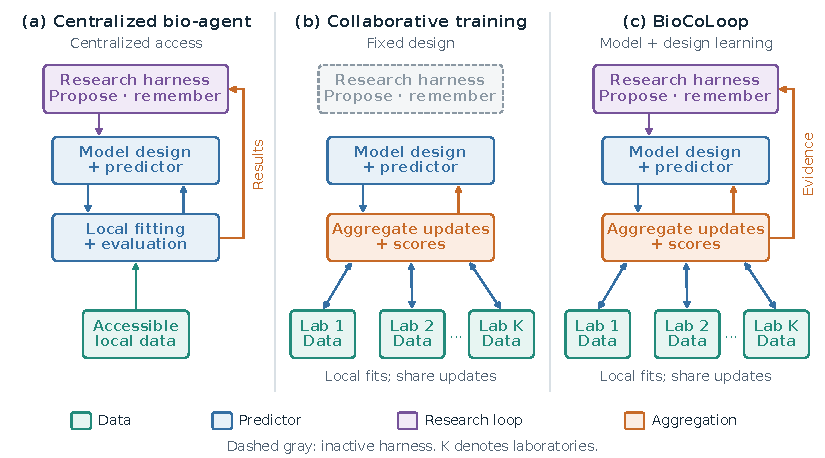
\includegraphics[width=\linewidth]{assets/paradigm_comparison.pdf}
\caption{
Research settings for biological AI.
A centralized bio-agent revises a model using centrally accessible data.
Collaborative training allows $K$ laboratories to optimize the same model and training configuration by sharing model updates rather than raw data.
BioCoLoop additionally uses results from local evaluation to guide subsequent changes to the model and training configuration.
}
\label{fig:paradigms}
\end{figure}
Our contributions are summarized as:
\begin{itemize}
\setlength{\parskip}{4pt}

\item We introduce BioCoLoop, a collaborative research framework that extends collaboration from parameter fitting to model development itself, allowing multiple laboratories to contribute without centralizing their raw data.

\item We develop a two-level procedure with an inner loop for collaborative training and evaluation and an outer loop for model development. Evaluation results from the inner loop are used to determine what model structure or training hyperparameters to test next, and which models should receive further training.

\item We validate the effectiveness of BioCoLoop on diverse scenarios, including drug--target interaction prediction, observed-response proteomic efficacy prediction, and cell perturbation identification. We further show that, with the same total amount of training and evaluation, using early evaluation results to decide which models continue training can improve performance.

\end{itemize}


\section*{2. Related work}
\paragraph{Collaborative learning for biological data.}
Parameter aggregation enables institutions to train a shared model while retaining their measurements locally \citep{McMahan2017,Sheller2020}. In single-cell analysis, scFed addresses cell-type classification and FedscGen addresses distributed batch correction \citep{Wang2024scFed,Bakhtiari2025FedscGen}. Tabula and its Chiron implementation support collaborative single-cell foundation-model training through an agent-enabled platform \citep{Ding2026Tabula,ChironCode}. Automated design can interact with local training: FedEx tunes hyperparameters while training shared weights \citep{Khodak2021FedEx}, and Helmsman synthesizes collaborative-learning systems through planning, coding and simulation-based refinement \citep{Li2025Helmsman}.

\paragraph{Self-improving agents in biological research.}
Self-improving agents turn experiment outcomes into subsequent computational proposals. AIDE searches candidate programs through drafting, debugging and improvement \citep{Jiang2025AIDE}, while the AI Scientist and AI-Scientist-v2 connect ideas to executed experiments, replanning, tree search and writing \citep{Lu2024AIScientist,Yamada2025AIScientistV2}. DrugEvolve combines research, implementation, evaluation and algorithm memory for drug-development tasks \citep{Zhou2026DrugEvolve,DrugEvolveCode}. BioCoLoop studies how multiple data-owning laboratories can supply development feedback through a shared research interface. TAPB, a ProteinTalks-derived efficacy head and scDEBART-based cell representations provide its task-specific prediction components \citep{lin2025tapb,Sun2026ProteinTalks,sung2026scdebart}. The proposal schema, fitting service and selection mechanism are common across tasks. Strong simple references on some perturbation benchmarks motivate evaluating the research procedure with fixed task predictors \citep{ahlmann2025linear}. Configuration search also connects to random search \citep{bergstra2012random}, Bayesian optimization \citep{snoek2012practical} and language-model proposal distributions \citep{yang2024opro}. We use feedback-free direct search to isolate the effect of development history under a shared proposal and fitting interface.

BioCoLoop connects collaborative fitting to a persistent development history. A shared coordinator executes candidate configurations across laboratories, aggregates their development measurements and returns structured evidence to a proposal model whose weights remain fixed. This interface supports history-guided proposal revision (Section 3.3) and, in a separate study, trajectory-guided training allocation (Section 3.4).


\section*{3. Method: federated evidence-guided research}
\subsection*{3.1 Two levels of model improvement}
The research object is an executable design $a$. A task adapter fixes the writable source interface, trainer, evaluation roles and resource budget. For predictor $f_{a,w}$, research has two levels:
\[
 w_a^{\mathcal K}=\operatorname{Fit}(a,\{D_i\}_{i\in\mathcal K}),
 \qquad
 a_{t+1}=\operatorname{Retain}(a_t,\widetilde a_t,E_t),
\]
where $\mathcal K$ denotes participating clients, $\widetilde a_t$ a proposed source change, and $E_t$ its measured development evidence. The inner procedure learns task weights; the outer procedure changes the representation, interaction module or policy. Fixed-predictor program search changes the prediction rule without new weight fitting. The research LLM remains fixed.

\begin{figure}[t]
\centering
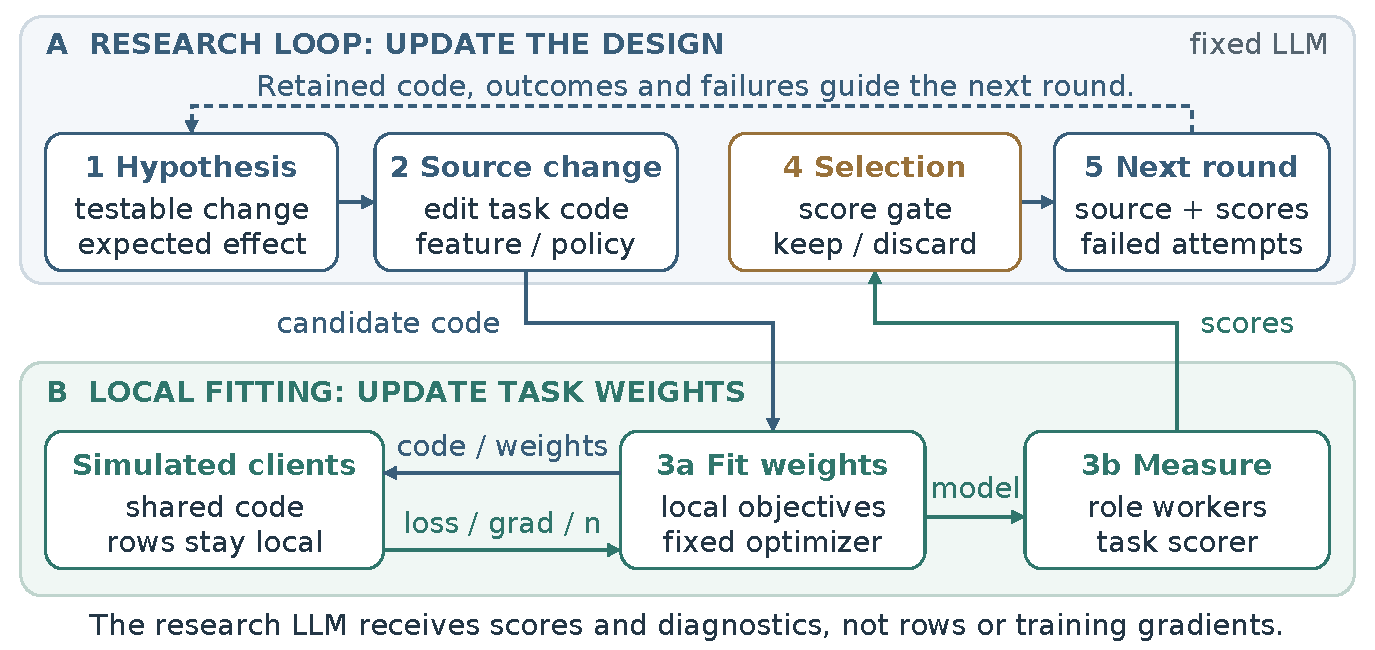
\includegraphics[width=\linewidth]{assets/method_diagram.pdf}
\caption{End-to-end pipeline. (A) Hypothesize, implement, evaluate, retain and revise. (B) Simulated clients keep separate response datasets and return gradients (proteomics) or fitted head weights (cell pilots); only evaluation summaries reach the LLM. (C) Task adapters share the research interface, not their training mode or metrics. DTI remains a centralized training/transfer study.}
\label{fig:research-interface}
\end{figure}

\subsection*{3.2 Hypotheses become measured source changes}
At round $t$, the proposer uses the task contract, shared agenda, retained source and scores, and accepted/rejected/failed history to state one change, its rationale and expected effect. Implementation edits only permitted source; interface checks precede fitting and scoring, and repairs consume the common budgets. Rejection updates the evidence, not the incumbent: subsequent proposals can learn from a failed change without inheriting it.

Retention requires both declared criteria to improve by more than $10^{-4}$: development/gate AP for the initial proteomics study, pooled out-of-fold/minimum-fold AP for its CV revision, and two validation-half AUROCs for fixed-predictor DTI. Native assessments cannot override this numerical selector. Harness-free generation uses the same task and selector but emits candidates directly, without separate hypothesis, implementation, review or memory stages.

Measured native loop attempts link hypothesis, source diff, parent, evaluator receipt, scores and decision. Failures inform subsequent proposals through separate receipts and need not appear in matched measurement history. These links expose what ran, why it was retained and which source was inherited. Native direct candidates omit separate hypotheses. The new bounded cell prototype instead shares a proposal format and varies feedback access (Appendix Q). Source inspection establishes the computation; measured outcomes, not the LLM's explanation, test its effect.

\subsection*{3.3 Local training and evidence transfer}
In the proteomics training adapter, $a$ specifies a stateless feature map $\phi_a$. Each client evaluates it on local protein responses and compound features. With $z=w^\top\phi_a(x)+b$, the fixed inner objective is logistic loss with coefficient penalty:
\[
 F_a(w,b)=\frac{1}{N}\left[\sum_{i\in\mathcal K}\sum_{(x,y)\in D_i}
 \bigl\{\log(1+e^z)-yz\bigr\}+\frac{\|w\|_2^2}{2C}\right],
 \quad N=\sum_{i\in\mathcal K}|D_i|,\ C=1.
\]
The coordinator aggregates local losses, gradients and counts for fixed L-BFGS-B updates (Figure~\ref{fig:research-interface}B). Source specifies \emph{what to fit}; client replies determine \emph{the weights}; evaluation summaries determine \emph{what to revise}. Evaluation workers receive source and fitted parameters and return aggregate scores. Training RPCs exclude raw arrays; the LLM receives neither rows nor gradients. For fixed source and clients, additivity recovers the centralized objective and gradient; Appendix K verifies equivalence. This existing optimizer lets research test changing representations with local data.

The historical evidence-only adapters instead train centrally and use partner diagnostics without adding partner training examples. Appendices C and N distinguish those studies from actual local-gradient training.

The biological motivation is access to complementary measurements under sharing constraints \citep{Sheller2020}. Direct generation receives the same client access as the loop within each condition. Crossing both controllers with one and ten clients separates research organization from data availability; fixed-feature references isolate the latter effect without source search.

\subsection*{3.4 Execution boundary}
The original source-search workers deny file opens, networking and new processes after initialization; fixed scorers, trainers and orchestration are trusted. The new cell prototype instead accepts bounded configurations and runs persistent client workers, without claiming an adversarial filesystem sandbox. It averages locally trained head parameters with FedAvg. Offline packaging simulates institutions on one host; fitting exchanges updates and scalar summaries, not raw responses. Neither implementation provides differential privacy or secure aggregation. Direct and loop arms share the boundary within each study.


\section*{4. Experiments}
\subsection*{4.1 Tasks, datasets and evaluation}

We evaluate BioCoLoop on three biological prediction problems. Each task uses its own base model, while collaborative training, evaluation, and proposal generation follow the same procedure. We consider two ways of forming laboratories. In the main setting, each dataset is divided into ten disjoint groups. In a complementary setting, distinct biological datasets or experimental scenarios are treated as separate laboratories. The first setting provides a controlled comparison of collaborative training, while the second tests whether information can transfer across genuinely different data sources.

\textbf{Drug-target interactions.}
Given a compound and a protein sequence, the model predicts whether they interact. BindingDB provides 50,149 training pairs and 5,604 development pairs, with canonical compounds defining laboratory assignments. We use TAPB as the base model, with frozen ESM2 protein features and trainable drug, fusion, and classification modules \citep{lin2025tapb}. The primary metric is AUROC on 5,505 random test pairs. Additional test sets containing 3,791 unseen-drug pairs and 2,507 unseen-protein pairs measure generalization to unseen entities. AP, MCC, accuracy, and cross-entropy are reported as secondary metrics.

\textbf{Observed-response proteomics.}
Given a drug representation and its measured 6h and 24h proteomic responses, the model predicts binary efficacy. A ProteinTalks PTPC subset provides 386 training, 105 development, and 148 test conditions \citep{Sun2026ProteinTalks}. Compound-group assignment gives each laboratory 49-50 training and development conditions. The base model is a ProteinTalks-derived efficacy model with protein and drug branches, trained from random initialization. Average precision (AP) is the primary metric. AUROC, accuracy, and cross-entropy are secondary metrics. Unlike de novo response prediction, this task conditions on observed post-treatment proteomic measurements.

\textbf{Cell perturbation identification.}
Given an expression response and five candidate interventions, the model identifies the intervention whose predicted response has the highest cosine similarity to the observation. We use VCC single-gene perturbations \citep{arc2025vcc}, Norman double-gene perturbations \citep{norman2019genetic}, and a Tahoe subset of drug perturbations in A549 at 5 $\mu$M \citep{zhang2025tahoe}. Intervention-disjoint training, development, and test counts are 60/20/20, 70/20/27, and 180/60/67, respectively. The base model uses a frozen scDEBART backbone with a trainable response head \citep{sung2026scdebart}. All methods use the same corrected attention masks and the same candidate sets. The primary metric is intervention-macro Top-1, which first averages accuracy within each intervention and then across interventions. Random selection has an expected Top-1 of 20\%. Micro Top-1, MRR, Top-3, and cross-entropy are reported as secondary metrics. Appendix A provides the response construction, chemical conditioning, training losses, and secondary evaluation details.

\subsection*{4.2 Compared methods and shared protocol}

\textbf{Compared methods.}
The \emph{fixed model} trains the task-specific base model with a fixed training recipe. \emph{Direct optimization} uses a self-improving model to propose changes to the model structure or training hyperparameters without access to results from previous experiments. AI-Scientist-v2 and AI-Researcher are adapted to the same biological tasks and evaluate their proposed changes through the same training and scoring procedure. BioCoLoop additionally provides results from completed experiments when generating subsequent proposals and performs collaborative training and evaluation across laboratories. We repeat the comparison with Qwen2.5-7B-Instruct and GPT-5.6 Luna as proposal generators. Details of the AI-Scientist-v2 and AI-Researcher adaptations are given in Appendix C.

The fixed, direct, AI-Scientist-v2, and AI-Researcher baselines use laboratory 0 because these methods do not support collaborative training and evaluation. BioCoLoop uses ten laboratories. The main table therefore compares complete systems rather than isolating the effect of laboratory access. To separate these effects, Appendix A reports a matched comparison that crosses fixed, direct, and BioCoLoop-style proposal generation with one or ten laboratories.

\textbf{Shared protocol.}
Direct optimization and BioCoLoop use the same twelve predefined combinations of model structure and training hyperparameters, the same six proposals, and the same first proposal. Each proposed model starts from the same task and seed-specific initialization and is trained for 100 rounds. Evaluation is performed every five rounds. Model selection averages the primary metric equally across participating laboratories. We report mean and sample standard deviation over seeds 42-44 using fixed data partitions. All methods within a task use the same held-out test set and evaluation code. Appendix A provides the complete training settings, matched comparisons, and uncertainty estimates.

% \subsection*{4.1 Tasks, datasets and evaluation}
% We study three biological prediction problems, using a separate predictor for each task and the same BioCoLoop research interface. The main comparison uses ten simulated laboratories formed by disjoint groups within each dataset. A complementary source-as-laboratory study assigns different biological collections or scenarios to separate laboratories. The first setting controls access to data; the second tests transfer between data sources.

% \paragraph{Drug--target interactions.}
% Given a compound and a protein sequence, the predictor estimates whether they interact. BindingDB supplies 50,149 training and 5,604 development pairs; canonical compounds define the laboratory assignments. The reference is TAPB with frozen ESM2 protein features and trainable drug, fusion and classification modules \citep{lin2025tapb}. The main endpoint is AUROC on 5,505 random-test pairs. Tests with 3,791 unseen-drug and 2,507 unseen-protein pairs assess entity generalization. AP, MCC, accuracy and cross-entropy provide secondary measures.

% \paragraph{Observed-response proteomics.}
% Given a drug representation and its measured 6h/24h proteomic response, the predictor estimates binary efficacy. A ProteinTalks PTPC subset supplies 386 training, 105 development and 148 test conditions \citep{Sun2026ProteinTalks}. Compound-group assignment gives each laboratory 49--50 training-plus-development conditions. The reference is a ProteinTalks-derived efficacy head with protein and drug branches, fitted from random initialization. Average precision (AP) is primary; AUROC, accuracy and cross-entropy are secondary. This task uses observed post-treatment measurements, rather than predicting efficacy from an unmeasured proteome.

% \paragraph{Cell perturbation identification.}
% Given an expression response and five candidate interventions, the model identifies the intervention whose predicted response has the highest cosine agreement with the observation. We use VCC single-gene perturbations \citep{arc2025vcc}, Norman double-gene perturbations \citep{norman2019genetic}, and a Tahoe subset of drug perturbations in A549 at 5 $\mu$M \citep{zhang2025tahoe}. Intervention-disjoint training/development/test counts are 60/20/20, 70/20/27 and 180/60/67, respectively. The reference is a frozen scDEBART backbone with a trainable response head \citep{sung2026scdebart}. All arms use the same corrected attention-mask implementation and fixed candidate rosters. Primary scoring is intervention-macro Top-1: accuracy is first averaged within each intervention, then across interventions. Random choice has expectation 20\%. Micro Top-1, MRR, Top-3 and cross-entropy are secondary. Appendix A describes response construction, chemical conditioning, losses and secondary metrics.

% \subsection*{4.2 Compared methods and shared protocol}
% The \emph{fixed model} trains each reference architecture with a fixed recipe on preselected laboratory 0. \emph{Direct optimization} proposes recipes without evaluation history, while AI-Scientist-v2 and AI-Researcher are task-adapted re-implementations that keep their native proposal logic but route candidates through the registered design interface on laboratory 0, with code execution, retrieval and manuscript generation disabled (Appendix~C). \emph{BioCoLoop} supplies evidence-card feedback to the proposer while training across ten laboratories. The main comparison repeats these methods in two research-model blocks, local Qwen2.5-7B-Instruct and GPT-5.6 Luna at low reasoning effort. A six-arm factorial comparison crosses fixed/direct/loop research with one/ten laboratories to separate data access from proposal feedback.

% Direct and loop search share a twelve-design library, six proposal slots and the first proposal. Every candidate starts from the same task/seed initialization and receives 100 training rounds, with development evaluation every five rounds. Selection uses equal-weight development scores over participating laboratories. The main results report mean and sample SD over seeds 42--44 on fixed data partitions. All methods within a task share the held-out test set and scorer. Appendix A gives the full factorial comparison, complete optimization settings and uncertainty estimates.

% Task-adapted AI-Scientist-v2 and AI-Researcher \citep{Yamada2025AIScientistV2,Tang2025AIResearcher} access laboratory 0 because they do not implement collaborative fitting or distributed evaluation, while BioCoLoop uses ten. All rows share the design library, candidate budget, training schedule and scorer. Qwen decoding uses registered generation seeds; the Luna service exposes no generation seed, so its seed labels identify training/search repetitions rather than deterministic sampling. Appendix~A separates loop and participation effects; Appendix~C details the adaptations.


\section*{5. Results}
\subsection*{5.1 Four-arm cell-policy comparison}
\begin{center}\footnotesize\setlength{\tabcolsep}{3pt}
\begin{tabularx}{\linewidth}{>{\hsize=1.600\hsize\linewidth=\hsize\raggedright\arraybackslash}X>{\hsize=0.800\hsize\linewidth=\hsize\raggedright\arraybackslash}X>{\hsize=0.800\hsize\linewidth=\hsize\raggedright\arraybackslash}X>{\hsize=0.800\hsize\linewidth=\hsize\raggedright\arraybackslash}X}
\toprule
Method & Reverse-ID Top-1 \(\uparrow\) & Sequential AUC3 \(\uparrow\) & CEX AURB3 \(\uparrow\) \\
\midrule
Our harness & 0.803922 & 0.723917 & 0.096127 \\
Our harness + federated evidence & 0.725490 & 0.723470 & 0.096127 \\
Harness-free & 0.764706 & 0.719532 & 0.096127 \\
Cosine baseline & 0.705882 & 0.721687 & N/A \\
\bottomrule
\end{tabularx}
\end{center}
Table 1. Exploratory cell-policy diagnostics, one campaign per task/method. The three metrics have different meanings and are not averaged.

Our harness records 41/51 reverse-identification hits, compared with 39/51 for direct and 36/51 for cosine. Sequential AUC3 improves by 0.004386 over direct, while the CEX learning arms have identical scores and executed-action hashes. The original Sequential confidence intervals compare policies with locked cosine, not harness with direct, and include zero for every learning arm. CEX's raw-PG reference is -0.007481; the shared learning-arm gain is 0.103608, with an original-scorer query-bootstrap 95\% interval of [0.068579, 0.139368]. This relative-objective improvement is shared by all three learning arms and is not harness-specific. Its absolute-response secondary objective worsens, so the result does not establish uniform drug-response benefit. Query-level replay intervals do not quantify variation across independent searches or biological laboratories.

The same-data federated variant does not outperform our non-federated harness. Across the three tasks, the latter uses 79 model calls and scores 17/18 candidates; the federated arm uses 87 calls and also scores 17/18; direct uses 18 calls and scores 9/18, with its other generations timing out at 900 seconds. These differences motivate the controlled DTI comparison, rather than an unsupported attribution of all score gains to research organization.

\subsection*{5.2 DTI held-out comparison}
\begin{center}\footnotesize\setlength{\tabcolsep}{3pt}
\begin{tabularx}{\linewidth}{>{\hsize=1.600\hsize\linewidth=\hsize\raggedright\arraybackslash}X>{\hsize=0.800\hsize\linewidth=\hsize\raggedright\arraybackslash}X>{\hsize=0.800\hsize\linewidth=\hsize\raggedright\arraybackslash}X>{\hsize=0.800\hsize\linewidth=\hsize\raggedright\arraybackslash}X}
\toprule
Method & Random AUROC & Unseen-drug AUROC & Unseen-protein AUROC \\
\midrule
DrugBAN & 0.8942 \(\pm\) 0.0230 & 0.8850 \(\pm\) 0.0317 & 0.8008 \(\pm\) 0.0734 \\
Released DrugBAN-Evo & 0.8715 \(\pm\) 0.0253 & 0.8612 \(\pm\) 0.0334 & 0.7181 \(\pm\) 0.0777 \\
Harness-free & 0.8950 \(\pm\) 0.0270 & 0.8853 \(\pm\) 0.0382 & 0.7958 \(\pm\) 0.0917 \\
Native DrugEvolve & 0.8963 \(\pm\) 0.0217 & 0.8865 \(\pm\) 0.0329 & 0.7975 \(\pm\) 0.0726 \\
Our harness & 0.9005 \(\pm\) 0.0207 & 0.8922 \(\pm\) 0.0299 & 0.8098 \(\pm\) 0.0678 \\
Cosine 5-NN (additional reference) & 0.8843 & 0.8719 & 0.7813 \\
\bottomrule
\end{tabularx}
\end{center}
Table 2. Neural rows use the fixed twelve-epoch refit, mean \(\pm\) sample SD over seeds 42--46; each searched row has five campaigns. All selected architectures completed refit without fallback and were sealed before testing. The additional deterministic cosine reference uses the identical 8,192 training pairs but was added retrospectively after the original tests; it has no training-seed SD.

Our harness has the highest observed mean AUROC on all three splits, above the fixed cosine reference. Primary differences are positive/negative/tied in 3/1/1 seeds against native DrugEvolve and 2/2/1 against direct generation. Both mean differences are below the predeclared 0.01 AUROC practical threshold, with intervals crossing zero (Table 3): a small, seed-dependent gain, not established superiority.

\begin{center}\footnotesize\setlength{\tabcolsep}{3pt}
\begin{tabularx}{\linewidth}{>{\hsize=1.600\hsize\linewidth=\hsize\raggedright\arraybackslash}X>{\hsize=0.850\hsize\linewidth=\hsize\raggedright\arraybackslash}X>{\hsize=0.850\hsize\linewidth=\hsize\raggedright\arraybackslash}X>{\hsize=0.850\hsize\linewidth=\hsize\raggedright\arraybackslash}X>{\hsize=0.850\hsize\linewidth=\hsize\raggedright\arraybackslash}X}
\toprule
Primary paired contrast & AUROC delta & 95\% bootstrap interval & Exact p & Holm p \\
\midrule
Our harness - Native DrugEvolve & +0.0057 & [-0.0174, +0.0280] & 0.6250 & 1.0000 \\
Our harness - Harness-free & +0.0069 & [-0.0147, +0.0326] & 0.7500 & 1.0000 \\
\bottomrule
\end{tabularx}
\end{center}
Table 3. Predeclared unseen-drug endpoint; paired campaign bootstrap and two-sided exact sign-flip tests (n=5).

Fixed-model variation reflects training seeds; searched-method variation also includes uncontrolled model generation. Secondary splits test transfer of selected architectures, not additional independent task families. Actual costs and fixed-order audit cases appear in Appendix D; Table D1 separates common ceilings from realized usage.

\subsection*{5.3 Matched proteomics results}
All 42 declared method/seed records are evaluated after both seals, with
35 unique prediction artifacts and no omitted seed or final-inference failure.
The final role contains 148 conditions, including 22 positives. Table 4
reports every searched arm and fixed reference; Appendix G gives all seed
values and secondary metrics.

\begin{table}[t]
% Generated from completed, independently rescored final results.
% results_sha256=e234c54386e4cda395d3273a992906595c436afce82799645709755b7139682c
\begin{center}\small\setlength{\tabcolsep}{7pt}
\begin{tabular}{lcc}
\toprule
Method & Final AP $\uparrow$ & Final AUROC $\uparrow$ \\
\midrule
Our harness (pooled) & $0.1822 \pm 0.0320$ & $0.5328 \pm 0.0488$ \\
Our harness + client cards & $0.1652 \pm 0.0157$ & $0.5034 \pm 0.0424$ \\
Harness-free (pooled) & $0.1926 \pm 0.0240$ & $0.5487 \pm 0.0371$ \\
Harness-free + client cards & $0.2002 \pm 0.0463$ & $0.5344 \pm 0.0774$ \\
Fixed efficacy head & $0.1589 \pm 0.0060$ & $0.4918 \pm 0.0224$ \\
Cosine 5-NN & $0.1685$ & $0.4989$ \\
Logistic regression & $0.1903$ & $0.6385$ \\
\bottomrule
\end{tabular}
\end{center}
Table N.4. Historical PTPC compound-disjoint final test, eight paired task-training seeds (mean $\pm$ sample SD). Cosine/logistic are deterministic references. Both pooled and cards arms access the same partner observations; cards add client-resolved diagnostics, including local AP/AUROC. The fixed head is our observed-response adaptation, not full ProteinTalks.

\end{table}

Harness-free+cards has the highest mean AP, 0.2002, compared with 0.1652
for our harness+cards. Their paired difference is $-0.0349$, with five
negative, two positive and one tied seed. Adding cards to our harness
also gives a negative mean difference, $-0.0170$. Neither predeclared
contrast supports the intended benefit (Table 5). The first descriptive
bootstrap interval is negative, but the exact Holm-adjusted test has
$p=0.125$; it does not establish multiplicity-corrected inferiority.

\begin{table}[t]
\begin{center}\footnotesize\setlength{\tabcolsep}{4pt}
\begin{tabular}{lcccc}
\toprule
AP contrast & Mean delta & 95\% interval & Exact p & Holm p \\
\midrule
Loop--direct (cards) & $-0.0349$ & $[-0.0623, -0.0101]$ & $0.0625$ & $0.1250$ \\
Cards--pooled (loop) & $-0.0170$ & $[-0.0429, +0.0028]$ & $0.4688$ & $0.4688$ \\
\bottomrule
\end{tabular}
\end{center}
Table N.5. Historical predeclared primary paired contrasts on AP. Intervals describe campaign variation conditional on this split; the practical threshold is 0.02 AP.

\end{table}

Absolute prediction quality is also limited. The neural methods' mean
AUROCs range from 0.4918 to 0.5487; logistic regression attains 0.6385
and BCE 0.4115, versus neural BCEs of 1.3719--1.4964. Logistic AP is
0.1903, above both loop variants. The final majority-class fraction is
126/148 (0.8514). Logistic attains exactly that accuracy by predicting every
condition negative at threshold 0.5; its ranking metrics use continuous
probabilities (Appendix J). Thus approximately 0.83 accuracy is not evidence
of strong efficacy discrimination. These results establish a completed observed-response
comparison with weak neural generalization, not an improvement over
ProteinTalks or a validated benefit from the federated diagnostic package.

\subsection*{5.4 Research cost and observed evidence transfer}
All 32 PTPC campaigns complete, with 128 successful fits, 640 client-worker receipts, 29 promotions and 67 rejections. Seven campaigns retain their starting head. Direct uses 24 calls per evidence mode; loop uses 85 with pooled diagnostics and 87 with cards. All input/output usage is observed. Loop therefore uses more calls and input tokens under the common ceilings; Tables H1--H2 report these costs separately from performance.

The fixed first-native cases give an executable example (Appendix H). In loop+pooled, seed 142, round 1, the proposal expects an explicit 24h-minus-6h representation to improve ranking. The code introduces shared per-time encoders, a difference branch and gated fusion. Visible dev/gate AP changes from 0.111316/0.630056 to 0.121785/0.752047, so the candidate is retained. Round 2 adds the drug embedding to the gate, expanding its input from 96 to 128; both AP values decrease, to 0.100287/0.727741, and the change is rejected. Round 3 inherits the retained source and explicitly cites the failed drug-conditioned gate before proposing head dropout. Source, decision, native-commit and next-context identities verify this sequence. It demonstrates recorded evidence transfer; held-out performance, rather than the generated explanation, determines method-level utility.


\section*{7. Conclusion}
AI4AI4Bio connects local biological measurements to shared model designs and fitted parameters. Improved designs reach DTI AUROC 0.9710/0.9588/0.9317 and proteomics AP 0.3727; ten-client access improves fixed-design AP by 6.11 points. Matched controls distinguish these gains from the variable effect of loop organization. Trainable perturbation-identification pilots extend the implementation, but require stronger adaptation before supporting a general performance claim.


\clearpage
\section*{Reproducibility and responsible use}
The accompanying release includes the pinned source commits, original-scorer hashes, search/refit contracts, all fifteen campaign terminal receipts, budgets, selected source hashes, checkpoints, row-aligned predictions, metric recomputation, seed-level tables, and failures. The final-test opening gate is a local manifest and procedural barrier; it is not cryptographic blinding against the machine owner. Model-call logs are text-only recorded invocations, and any observed CLI tool execution fails the call. The study involves existing offline benchmarks, not prospective wet-lab or clinical use. No generated prediction should be interpreted as validated therapeutic advice.

\clearpage
\bibliographystyle{iclr2027_conference}
\bibliography{references}
\clearpage


\clearpage
\section*{Appendix A. Uniform collaborative research protocol}
\label{app:unified}
\setcounter{table}{0}
\renewcommand{\thetable}{A.\arabic{table}}
\renewcommand{\theHtable}{A.\arabic{table}}
\makeatletter
\setlength{\@fptop}{0pt}
\makeatother

\paragraph{Versioned implementation.}
The reported study uses \texttt{core\_v3.py}, \texttt{run\_v3.py} and \texttt{research\_v2.py}. All task families execute the same optimization, aggregation, proposal and retention source through task-specific adapters. TAPB workers use the TAPB environment; Qwen, proteomics and cell adapters use the LDA environment. Each scientific fit starts from its task-specific public or random initialization, with no reuse of earlier task-trained weights.

\paragraph{Shared optimization and checkpoint selection.}
Each round uses one local AdamW epoch, batch size 64 and gradient-norm clipping at one; local optimizer state resets between rounds. Parameters are averaged with training-example weights. If server momentum is enabled, the coordinator multiplies the previous velocity by the configured momentum coefficient and adds the difference between the averaged parameters and the previous shared parameters, then adds that velocity to the shared parameters. Floating model buffers are averaged and integer buffers use an elementwise maximum. Momentum acts on trainable parameters only. Every full-training candidate runs for 100 rounds; local development scores are collected every five rounds. Checkpoint selection maximizes the equal-client primary score, then minimizes mean development loss. The optional residual adapter has width 32 and zero-initialized output. The DTI adapter trains TAPB using frozen public protein features, the proteomic adapter trains its efficacy head from random initialization, and the cell adapters train response heads on frozen corrected scDEBART features.

\paragraph{Complete design library.}
Each identifier below compiles to one executable candidate. D00 is the fixed starting recipe; D01--D11 are available to both direct and loop search without within-arm repetition. Six proposal slots define the common budget.

\begin{center}\small
\begin{tabular}{lrrrr}
\toprule
Design & Learning rate & Weight decay & Momentum & Residual adapter \\
\midrule
D00 & 0.001 & 0.001 & 0 & no \\
D01 & 0.0001 & 0.001 & 0 & no \\
D02 & 0.01 & 0.001 & 0 & no \\
D03 & 0.001 & 0 & 0 & no \\
D04 & 0.001 & 0.01 & 0 & no \\
D05 & 0.001 & 0.001 & 0.9 & no \\
D06 & 0.001 & 0.001 & 0 & yes \\
D07 & 0.001 & 0.001 & 0.9 & yes \\
D08 & 0.0001 & 0.001 & 0 & yes \\
D09 & 0.0001 & 0.001 & 0.9 & yes \\
D10 & 0.01 & 0.01 & 0 & no \\
D11 & 0.001 & 0.01 & 0 & yes \\
\bottomrule
\end{tabular}
\end{center}

\paragraph{Proposal generation and evidence memory.}
The main-study proposer is Qwen2.5-7B-Instruct, using bfloat16 inference, temperature 0.7, top-$p$ 0.9 and at most 512 new tokens. Each slot uses a deterministic seed derived from the training seed. Direct and loop comparisons share the same first proposal. Later direct proposals receive the default reference configuration and remaining untried identifiers, without evaluation scores. Loop proposals instead receive the latest retained configuration and ordered evidence cards, each containing the candidate configuration, aggregate best development metric and loss, best round, first/last training and validation records, and final status. A bounded second generation attempt repairs schema or novelty violations. Failed proposals consume a slot. Identical configurations within a seed and participation setting can reuse a completed fit while retaining their logical positions in the research traces.

Every proposal has the following executable JSON shape:
\begin{verbatim}
{
  "hypothesis": "one testable claim about an editable factor",
  "experiment": "the controlled change and incumbent comparison",
  "expected_effect": "the expected metric and diagnostic response",
  "design_id": "D00--D11"
}
\end{verbatim}
The compiler validates \texttt{design\_id} against the table above. The finalizer then attaches executed measurements and a retention decision to the proposal, creating the evidence card used in the next iteration.

\paragraph{Executed loop trajectories.}
Three ten-laboratory traces illustrate how the common finalizer operates. Values are aggregate development measurements on the 0--1 primary-metric scale, and proposal slots are one-indexed.

\begin{center}\small
\begin{tabular}{llrrl}
\toprule
Study & Selected design & Primary & Loss & First direct / loop slot \\
\midrule
PTPC, seed 42 & D04 & 0.665833 & 0.521161 & 5 / 5 \\
VCC, seed 43 & D00 & 0.240350 & 1.607792 & initial baseline \\
Norman, seed 42 & D08 & 0.519000 & 1.538505 & 3 / 2 \\
\bottomrule
\end{tabular}
\end{center}

PTPC selects stronger weight decay through the BCE tie-break at equal AP. VCC retains the initial design after six alternatives. On Norman, the loop reaches the winning lower-learning-rate residual design one slot before direct search. Across all 15 ten-laboratory task--seed trajectories, the two-proposal loop is better in two, tied in thirteen and worse in none; the mean development-primary difference is +0.78 percentage points. At six proposals, direct and loop select the same checkpoints, reflecting coverage saturation in the twelve-design library.

\paragraph{Compute-matched evidence racing.}
The follow-up feedback-isolation protocol uses a ten-design fractional-factorial slate and newly executed seeds 53--55. Direct search assigns 80 rounds to every design. The loop assigns 20 screening rounds to every design, stratifies candidates by learning rate, and promotes both the strongest current candidate and the fastest-improving candidate within each stratum. Six promoted candidates restart from the common initialization for 100-round validation. Consequently, each arm executes 800 full-client rounds and 160 development measurements over the same ten hypotheses. The promotion record is finalized before any held-out response is read.

Across the resulting 12 proteomics/cell held-out comparisons, racing gives four wins, eight ties and no losses. Norman improves by 10.84 Top-1 points on average, with seed-level effects of +10.00, +11.70 and +10.81 and a hierarchical paired-bootstrap 95\% interval of [4.54, 17.73]. Tahoe gives one +5.97-point seed and two ties; VCC and PTPC tie in all three seeds. Independent rescoring of every saved prediction reproduces the reported metrics exactly. A TAPB companion replay applies the same screen/promote principle to the seven-design intersection of existing traces: direct receives 525 candidate-rounds, the loop receives 520, and the development AUROC effect is +0.39 points on average (two wins, one tie).

\paragraph{Client and split integrity.}
DTI clients contain 4,932--5,058 training and 517--643 development pairs. Compound identities do not cross clients. The fixed test roles contain 5,505 random, 3,791 unseen-drug and 2,507 unseen-protein pairs. PTPC partitions 333 compound groups into 386 fitting and 105 development conditions, with 35--42 fitting conditions per client; its frozen test role contains 148 conditions. VCC, Norman and Tahoe use whole-intervention splits of 60/20/20, 70/20/27 and 180/60/67. Their ten clients own equal numbers of training and development intervention identities.

\paragraph{Proteomic preprocessing.}
For each 6h and 24h profile, the PTPC adapter applies log1p, within-profile min--max normalization over finite observations, zero filling and unit L2 normalization. The 2,048-bit Morgan vector is separately L2-normalized and scaled by 0.5. Concatenating the two 5,171-dimensional proteomic blocks with the drug vector produces a 12,390-dimensional float32 input. The ProteinTalks-derived efficacy head contains 464,193 parameters at D00. Every arm uses identical inputs, initialization policy, 100-round budget and checkpoint rule.

\paragraph{Full factorial results.}
The following tables report all six held-out arms, complete method contrasts, proposal-prefix analysis, secondary metrics, uncertainty and all three DTI test roles. Bold marks the best displayed value within each task and metric, including ties. Higher is better except BCE and cross-entropy.

\begin{table}[t]
\centering\small
\setlength{\tabcolsep}{3pt}
\begin{tabular}{clrrrrr}
\toprule
 & & DTI & Proteomics & \multicolumn{3}{c}{Cell perturbation} \\
\cmidrule(lr){5-7}
Labs & Method & AUROC & AP & VCC & Norman & Tahoe \\
 & & $\uparrow$ & $\uparrow$ & Top-1 $\uparrow$ & Top-1 $\uparrow$ & Top-1 $\uparrow$ \\
\midrule
1 & Fixed model & 81.76 & 25.05{\scriptsize$\pm4.56$} & 29.94{\scriptsize$\pm0.00$} & \textbf{25.56}{\scriptsize$\pm0.00$} & 19.40{\scriptsize$\pm0.00$} \\
1 & Direct & 88.82 & 20.13{\scriptsize$\pm0.07$} & 21.09{\scriptsize$\pm4.38$} & 14.15{\scriptsize$\pm0.00$} & 15.42{\scriptsize$\pm6.21$} \\
1 & Our loop & 88.82 & 20.13{\scriptsize$\pm0.07$} & 20.22{\scriptsize$\pm2.22$} & 14.15{\scriptsize$\pm0.00$} & 15.42{\scriptsize$\pm6.21$} \\
\midrule
10 & Fixed model & 94.27 & \textbf{37.07}{\scriptsize$\pm0.08$} & \textbf{31.54}{\scriptsize$\pm0.08$} & 15.48{\scriptsize$\pm0.00$} & \textbf{25.87}{\scriptsize$\pm1.72$} \\
10 & Direct & \textbf{94.60} & 36.99{\scriptsize$\pm0.22$} & \textbf{31.54}{\scriptsize$\pm0.08$} & 22.25{\scriptsize$\pm0.45$} & 22.39{\scriptsize$\pm2.59$} \\
10 & Our loop & \textbf{94.60} & 36.99{\scriptsize$\pm0.22$} & \textbf{31.54}{\scriptsize$\pm0.08$} & 22.25{\scriptsize$\pm0.45$} & 22.39{\scriptsize$\pm2.59$} \\
\midrule
\multicolumn{2}{l}{Completed seeds ($n/3$)} & 1/3 & 3/3 & 3/3 & 3/3 & 3/3 \\
\bottomrule
\end{tabular}
\caption{Six-arm ablation of the committed reference-model versions. Entries are completed-seed means and sample SD where at least two seeds are available. DTI uses the random held-out endpoint. Retrospective held-out means are multiplied by 100; completed seed counts are shown. Bold marks all displayed maxima. N/A denotes incomplete paired evaluation. Model versions were not selected by held-out scores; these endpoints are not blind confirmation.}
\label{tab:strong-ablation}
\end{table}

\begin{table}[t]
\centering\small
\setlength{\tabcolsep}{3pt}
\begin{tabular}{lrrrrr}
\toprule
Held-out contrast & DTI & Proteomics & VCC & Norman & Tahoe \\
\midrule
Loop $-$ fixed (1 lab) & N/A & -4.91 & -9.71 & -11.41 & -7.46 \\
Loop $-$ fixed (10 labs) & N/A & -0.08 & +0.00 & +6.81 & -1.49 \\
Loop $-$ direct (1 lab) & N/A & +0.00 & -0.87 & +0.00 & +0.00 \\
Loop $-$ direct (10 labs) & N/A & +0.00 & +0.00 & +0.00 & +0.00 \\
10 $-$ 1 labs (both fixed) & N/A & +12.02 & +1.61 & -10.07 & +5.97 \\
10 $-$ 1 labs (both direct) & N/A & +16.85 & +10.45 & +8.15 & +11.94 \\
10 $-$ 1 labs (both loop) & N/A & +16.85 & +11.32 & +8.15 & +11.94 \\
\midrule
Completed seeds ($n/3$) & 0/3 & 3/3 & 3/3 & 2/3 & 2/3 \\
\bottomrule
\end{tabular}
\caption{Separating total research/search improvement (loop minus fixed), feedback-specific improvement (loop minus matched-budget direct), and access to more laboratory data (ten minus one lab with loop fixed). Mean paired differences are in percentage points over the completed seeds on retrospective held-out data. Total search improvement must not be attributed solely to feedback. Negative effects and ties are retained; per-seed uncertainty is in Appendix R.}
\label{tab:strong-effects-full}
\end{table}

\begin{table}[t]
\centering\small
\setlength{\tabcolsep}{6pt}
\begin{tabular}{rrrrr}
\toprule
Proposal budget & Loop better & Tie & Direct better & Mean $\Delta$ primary \\
 & \multicolumn{3}{c}{task--seed trajectories} & points \\
\midrule
1 & 0 & 15 & 0 & +0.00 \\
2 & 2 & 13 & 0 & +0.78 \\
3 & 0 & 14 & 1 & -0.04 \\
4 & 0 & 15 & 0 & +0.00 \\
5 & 0 & 14 & 1 & -0.02 \\
6 & 0 & 15 & 0 & +0.00 \\
\bottomrule
\end{tabular}
\caption{Executed-prefix analysis of all 15 ten-laboratory development trajectories at common proposal budgets. At two proposals, feedback-guided search improves TAPB seed 44 by 4.84 points and Norman seed 42 by 6.90 points, with thirteen ties and no regressions.}
\label{tab:loop-prefix}
\end{table}

\clearpage
\begin{longtable}{llrrrr}
\caption{Held-out secondary metrics for the task-reference models, averaged over seeds 42--44 and multiplied by 100. Bold indicates all tied maxima, or minima for loss.}\label{tab:strong-secondary}\\
\toprule Method & Labs & Metric 1 & Metric 2 & Metric 3 & Metric 4 \\ \midrule\endfirsthead
\toprule Method & Labs & Metric 1 & Metric 2 & Metric 3 & Metric 4 \\ \midrule\endhead
\multicolumn{2}{l}{\textbf{DTI ($n=3$)}} & AUROC & AP & MCC & BCE \\
Fixed model & 1 & 82.83 & 81.57 & 49.95 & 52.37 \\
Direct & 1 & 89.89 & 87.77 & 65.71 & 61.02 \\
Our loop & 1 & 89.89 & 87.77 & 65.71 & 61.02 \\
Our loop & 10 & \textbf{93.76} & \textbf{92.73} & \textbf{73.71} & \textbf{36.59} \\
\midrule
\multicolumn{2}{l}{\textbf{Proteomics ($n=3$)}} & AP & AUROC & BCE & Acc. \\
Fixed model & 1 & 25.05 & 65.49 & 42.65 & \textbf{85.14} \\
Direct & 1 & 20.13 & 61.80 & 44.34 & 81.76 \\
Our loop & 1 & 20.13 & 61.80 & 44.34 & 81.76 \\
Our loop & 10 & \textbf{36.99} & \textbf{73.87} & \textbf{39.83} & \textbf{85.14} \\
\midrule
\multicolumn{2}{l}{\textbf{VCC ($n=3$)}} & Micro Top-1 & MRR & Top-3 & CE \\
Fixed model & 1 & 33.61 & \textbf{56.53} & \textbf{73.89} & \textbf{154.51} \\
Direct & 1 & 21.48 & 47.10 & 62.78 & 160.82 \\
Our loop & 1 & 20.74 & 46.94 & 64.26 & 160.86 \\
Our loop & 10 & \textbf{33.98} & 56.34 & 69.44 & 158.14 \\
\midrule
\multicolumn{2}{l}{\textbf{Norman ($n=3$)}} & Micro Top-1 & MRR & Top-3 & CE \\
Fixed model & 1 & \textbf{25.56} & 48.50 & 63.93 & \textbf{158.74} \\
Direct & 1 & 14.15 & 42.12 & 58.35 & 160.39 \\
Our loop & 1 & 14.15 & 42.12 & 58.35 & 160.39 \\
Our loop & 10 & 22.25 & \textbf{50.07} & \textbf{70.96} & 158.83 \\
\midrule
\multicolumn{2}{l}{\textbf{Tahoe ($n=3$)}} & Micro Top-1 & MRR & Top-3 & CE \\
Fixed model & 1 & 19.40 & 45.00 & 58.21 & 163.08 \\
Direct & 1 & 15.42 & 42.60 & 56.72 & 161.90 \\
Our loop & 1 & 15.42 & 42.60 & 56.72 & 161.90 \\
Our loop & 10 & \textbf{22.39} & \textbf{47.95} & \textbf{61.19} & \textbf{160.75} \\
\midrule
\bottomrule
\end{longtable}

\begin{longtable}{llrrl}
\caption{Per-seed paired cluster-bootstrap 95\% intervals for the committed model versions, in percentage points. These retrospective intervals condition on fixed trained models and do not measure across-seed uncertainty. DTI intervals, when available, are a post-hoc supplement using frozen predictions; random-endpoint rows use drug clusters.}\label{tab:strong-uncertainty}\\
\toprule Task & Contrast & Seed & Difference & 95\% interval \\ \midrule\endfirsthead
\toprule Task & Contrast & Seed & Difference & 95\% interval \\ \midrule\endhead
DTI & Loop $-$ fixed (10 labs) & 42 & +0.33 & [-0.06, +0.69] \\
DTI & Loop $-$ direct (1 lab) & 42 & +0.00 & [+0.00, +0.00] \\
DTI & Loop $-$ direct (10 labs) & 42 & +0.00 & [+0.00, +0.00] \\
DTI & 10 $-$ 1 labs (both fixed) & 42 & +12.51 & [+11.35, +13.71] \\
DTI & 10 $-$ 1 labs (both direct) & 42 & +5.78 & [+5.02, +6.57] \\
DTI & 10 $-$ 1 labs (both loop) & 42 & +5.78 & [+5.02, +6.57] \\
\midrule
DTI & Loop $-$ fixed (10 labs) & 43 & +0.54 & [-0.08, +1.11] \\
DTI & Loop $-$ direct (1 lab) & 43 & +0.00 & [+0.00, +0.00] \\
DTI & Loop $-$ direct (10 labs) & 43 & +0.00 & [+0.00, +0.00] \\
DTI & 10 $-$ 1 labs (both fixed) & 43 & +7.80 & [+6.82, +8.82] \\
DTI & 10 $-$ 1 labs (both direct) & 43 & +1.65 & [+0.90, +2.38] \\
DTI & 10 $-$ 1 labs (both loop) & 43 & +1.65 & [+0.90, +2.38] \\
\midrule
DTI & Loop $-$ fixed (10 labs) & 44 & +5.01 & [+4.25, +5.71] \\
DTI & Loop $-$ direct (1 lab) & 44 & +0.00 & [+0.00, +0.00] \\
DTI & Loop $-$ direct (10 labs) & 44 & +0.00 & [+0.00, +0.00] \\
DTI & 10 $-$ 1 labs (both fixed) & 44 & +6.60 & [+5.61, +7.74] \\
DTI & 10 $-$ 1 labs (both direct) & 44 & +4.17 & [+3.45, +4.93] \\
DTI & 10 $-$ 1 labs (both loop) & 44 & +4.17 & [+3.45, +4.93] \\
\midrule
Proteomics & Loop $-$ fixed (10 labs) & 42 & +0.00 & [+0.00, +0.00] \\
Proteomics & Loop $-$ direct (1 lab) & 42 & +0.00 & [+0.00, +0.00] \\
Proteomics & Loop $-$ direct (10 labs) & 42 & +0.00 & [+0.00, +0.00] \\
Proteomics & 10 $-$ 1 labs (both fixed) & 42 & +13.16 & [-0.39, +26.02] \\
Proteomics & 10 $-$ 1 labs (both direct) & 42 & +16.91 & [+3.37, +31.02] \\
Proteomics & 10 $-$ 1 labs (both loop) & 42 & +16.91 & [+3.37, +31.02] \\
\midrule
Proteomics & Loop $-$ fixed (10 labs) & 43 & +0.00 & [+0.00, +0.00] \\
Proteomics & Loop $-$ direct (1 lab) & 43 & +0.00 & [+0.00, +0.00] \\
Proteomics & Loop $-$ direct (10 labs) & 43 & +0.00 & [+0.00, +0.00] \\
Proteomics & 10 $-$ 1 labs (both fixed) & 43 & +15.98 & [+1.29, +29.00] \\
Proteomics & 10 $-$ 1 labs (both direct) & 43 & +17.03 & [+3.34, +31.44] \\
Proteomics & 10 $-$ 1 labs (both loop) & 43 & +17.03 & [+3.34, +31.44] \\
\midrule
Proteomics & Loop $-$ fixed (10 labs) & 44 & -0.24 & [-3.40, +2.33] \\
Proteomics & Loop $-$ direct (1 lab) & 44 & +0.00 & [+0.00, +0.00] \\
Proteomics & Loop $-$ direct (10 labs) & 44 & +0.00 & [+0.00, +0.00] \\
Proteomics & 10 $-$ 1 labs (both fixed) & 44 & +6.93 & [-3.43, +15.60] \\
Proteomics & 10 $-$ 1 labs (both direct) & 44 & +16.63 & [+3.02, +31.08] \\
Proteomics & 10 $-$ 1 labs (both loop) & 44 & +16.63 & [+3.02, +31.08] \\
\midrule
VCC & Loop $-$ fixed (10 labs) & 42 & +0.00 & [+0.00, +0.00] \\
VCC & Loop $-$ direct (1 lab) & 42 & +0.00 & [+0.00, +0.00] \\
VCC & Loop $-$ direct (10 labs) & 42 & +0.00 & [+0.00, +0.00] \\
VCC & 10 $-$ 1 labs (both fixed) & 42 & +1.70 & [-5.36, +8.58] \\
VCC & 10 $-$ 1 labs (both direct) & 42 & +9.90 & [-2.88, +23.04] \\
VCC & 10 $-$ 1 labs (both loop) & 42 & +9.90 & [-2.88, +23.04] \\
\midrule
VCC & Loop $-$ fixed (10 labs) & 43 & +0.00 & [+0.00, +0.00] \\
VCC & Loop $-$ direct (1 lab) & 43 & +4.83 & [-5.50, +16.49] \\
VCC & Loop $-$ direct (10 labs) & 43 & +0.00 & [+0.00, +0.00] \\
VCC & 10 $-$ 1 labs (both fixed) & 43 & +1.56 & [-5.76, +8.58] \\
VCC & 10 $-$ 1 labs (both direct) & 43 & +15.08 & [+2.94, +27.78] \\
VCC & 10 $-$ 1 labs (both loop) & 43 & +10.24 & [-2.74, +23.49] \\
\midrule
VCC & Loop $-$ fixed (10 labs) & 44 & +0.00 & [+0.00, +0.00] \\
VCC & Loop $-$ direct (1 lab) & 44 & -7.44 & [-17.23, +1.33] \\
VCC & Loop $-$ direct (10 labs) & 44 & +0.00 & [+0.00, +0.00] \\
VCC & 10 $-$ 1 labs (both fixed) & 44 & +1.56 & [-5.76, +8.58] \\
VCC & 10 $-$ 1 labs (both direct) & 44 & +6.38 & [-4.38, +19.13] \\
VCC & 10 $-$ 1 labs (both loop) & 44 & +13.82 & [+2.54, +26.34] \\
\midrule
Norman & Loop $-$ fixed (10 labs) & 42 & +7.26 & [-9.41, +25.41] \\
Norman & Loop $-$ direct (1 lab) & 42 & +0.00 & [+0.00, +0.00] \\
Norman & Loop $-$ direct (10 labs) & 42 & +0.00 & [+0.00, +0.00] \\
Norman & 10 $-$ 1 labs (both fixed) & 42 & -10.07 & [-21.19, +0.00] \\
Norman & 10 $-$ 1 labs (both direct) & 42 & +8.59 & [-8.30, +26.00] \\
Norman & 10 $-$ 1 labs (both loop) & 42 & +8.59 & [-8.30, +26.00] \\
\midrule
Norman & Loop $-$ fixed (10 labs) & 43 & +6.37 & [-11.12, +24.81] \\
Norman & Loop $-$ direct (1 lab) & 43 & +0.00 & [+0.00, +0.00] \\
Norman & Loop $-$ direct (10 labs) & 43 & +0.00 & [+0.00, +0.00] \\
Norman & 10 $-$ 1 labs (both fixed) & 43 & -10.07 & [-21.19, +0.00] \\
Norman & 10 $-$ 1 labs (both direct) & 43 & +7.70 & [-9.33, +25.85] \\
Norman & 10 $-$ 1 labs (both loop) & 43 & +7.70 & [-9.33, +25.85] \\
\midrule
Norman & Loop $-$ fixed (10 labs) & 44 & +6.67 & [-10.37, +24.81] \\
Norman & Loop $-$ direct (1 lab) & 44 & +0.00 & [+0.00, +0.00] \\
Norman & Loop $-$ direct (10 labs) & 44 & +0.00 & [+0.00, +0.00] \\
Norman & 10 $-$ 1 labs (both fixed) & 44 & -10.07 & [-21.19, +0.00] \\
Norman & 10 $-$ 1 labs (both direct) & 44 & +8.00 & [-8.52, +25.93] \\
Norman & 10 $-$ 1 labs (both loop) & 44 & +8.00 & [-8.52, +25.93] \\
\midrule
Tahoe & Loop $-$ fixed (10 labs) & 42 & +0.00 & [+0.00, +0.00] \\
Tahoe & Loop $-$ direct (1 lab) & 42 & +0.00 & [+0.00, +0.00] \\
Tahoe & Loop $-$ direct (10 labs) & 42 & +0.00 & [+0.00, +0.00] \\
Tahoe & 10 $-$ 1 labs (both fixed) & 42 & +4.48 & [-5.97, +14.93] \\
Tahoe & 10 $-$ 1 labs (both direct) & 42 & +10.45 & [-1.49, +22.39] \\
Tahoe & 10 $-$ 1 labs (both loop) & 42 & +10.45 & [-1.49, +22.39] \\
\midrule
Tahoe & Loop $-$ fixed (10 labs) & 43 & -2.99 & [-7.46, +0.00] \\
Tahoe & Loop $-$ direct (1 lab) & 43 & +0.00 & [+0.00, +0.00] \\
Tahoe & Loop $-$ direct (10 labs) & 43 & +0.00 & [+0.00, +0.00] \\
Tahoe & 10 $-$ 1 labs (both fixed) & 43 & +7.46 & [-4.48, +17.95] \\
Tahoe & 10 $-$ 1 labs (both direct) & 43 & +13.43 & [+1.49, +23.88] \\
Tahoe & 10 $-$ 1 labs (both loop) & 43 & +13.43 & [+1.49, +23.88] \\
\midrule
Tahoe & Loop $-$ fixed (10 labs) & 44 & -7.46 & [-19.40, +4.48] \\
Tahoe & Loop $-$ direct (1 lab) & 44 & +0.00 & [+0.00, +0.00] \\
Tahoe & Loop $-$ direct (10 labs) & 44 & +0.00 & [+0.00, +0.00] \\
Tahoe & 10 $-$ 1 labs (both fixed) & 44 & +7.46 & [-4.48, +17.95] \\
Tahoe & 10 $-$ 1 labs (both direct) & 44 & -2.99 & [-17.91, +11.94] \\
Tahoe & 10 $-$ 1 labs (both loop) & 44 & -2.99 & [-17.91, +11.94] \\
\midrule
\bottomrule
\end{longtable}

\begin{longtable}{llrrr}
\caption{All three frozen TAPB held-out endpoints under the committed common protocol. Scores are completed-seed means multiplied by 100; N/A means no complete independently verified six-arm evaluation. The main DTI endpoint is random held-out.}\label{tab:strong-dti-endpoints}\\
\toprule Endpoint & Method & Labs & AUROC & AP \\ \midrule\endfirsthead
\toprule Endpoint & Method & Labs & AUROC & AP \\ \midrule\endhead
Random & Fixed model & 1 & 81.76 & 82.30 \\
Random & Direct & 1 & 88.82 & 85.98 \\
Random & Our loop & 1 & 88.82 & 85.98 \\
Random & Fixed model & 10 & 94.27 & 92.87 \\
Random & Direct & 10 & \textbf{94.60} & \textbf{94.27} \\
Random & Our loop & 10 & \textbf{94.60} & \textbf{94.27} \\
\midrule
Unseen drug & Fixed model & 1 & 80.67 & 86.41 \\
Unseen drug & Direct & 1 & 86.68 & 87.08 \\
Unseen drug & Our loop & 1 & 86.68 & 87.08 \\
Unseen drug & Fixed model & 10 & 92.96 & 93.58 \\
Unseen drug & Direct & 10 & \textbf{93.06} & \textbf{94.63} \\
Unseen drug & Our loop & 10 & \textbf{93.06} & \textbf{94.63} \\
\midrule
Unseen protein & Fixed model & 1 & 69.86 & 78.05 \\
Unseen protein & Direct & 1 & 81.05 & 77.04 \\
Unseen protein & Our loop & 1 & 81.05 & 77.04 \\
Unseen protein & Fixed model & 10 & 89.88 & 86.19 \\
Unseen protein & Direct & 10 & \textbf{89.91} & \textbf{90.30} \\
Unseen protein & Our loop & 10 & \textbf{89.91} & \textbf{90.30} \\
\midrule
\bottomrule
\end{longtable}

\begingroup\scriptsize\setlength{\tabcolsep}{3pt}
\begin{longtable}{llrrrr}
\caption{Post-hoc TAPB uncertainty supplement from frozen prediction files. All three endpoints, six arms and fixed contrasts are retained. Entries are paired AUROC/AP differences and percentile 95\% intervals in percentage points from 1,000 requested cluster draws (RNG seed 20260918). Random and unseen-drug endpoints resample drug clusters; unseen-protein resamples protein clusters. Intervals condition on fixed trained models and one clustering axis; they are not two-way, across-seed, multiplicity-adjusted, or prospective confirmatory intervals.}\label{tab:strong-dti-uncertainty}\\
\toprule Endpoint / seed & Contrast & AUROC $\Delta$ & 95\% interval & AP $\Delta$ & 95\% interval \\ \midrule\endfirsthead
\toprule Endpoint / seed & Contrast & AUROC $\Delta$ & 95\% interval & AP $\Delta$ & 95\% interval \\ \midrule\endhead
Random / 42 & Loop $-$ fixed (10 labs) & +0.33 & [-0.06, +0.69] & +1.40 & [+0.76, +2.05] \\
Random / 42 & Loop $-$ direct (1 lab) & +0.00 & [+0.00, +0.00] & +0.00 & [+0.00, +0.00] \\
Random / 42 & Loop $-$ direct (10 labs) & +0.00 & [+0.00, +0.00] & +0.00 & [+0.00, +0.00] \\
Random / 42 & 10 $-$ 1 labs (fixed) & +12.51 & [+11.35, +13.71] & +10.56 & [+9.10, +12.11] \\
Random / 42 & 10 $-$ 1 labs (direct) & +5.78 & [+5.02, +6.57] & +8.29 & [+7.01, +9.56] \\
Random / 42 & 10 $-$ 1 labs (loop) & +5.78 & [+5.02, +6.57] & +8.29 & [+7.01, +9.56] \\
Random / 42 & Our harness $-$ fixed (1 lab) & +12.84 & [+11.82, +14.01] & +11.96 & [+10.56, +13.45] \\
Random / 42 & Our harness $-$ direct (1 lab) & +5.78 & [+5.02, +6.57] & +8.29 & [+7.01, +9.56] \\
\midrule
Unseen drug / 42 & Loop $-$ fixed (10 labs) & +0.10 & [-0.47, +0.67] & +1.06 & [+0.42, +1.66] \\
Unseen drug / 42 & Loop $-$ direct (1 lab) & +0.00 & [+0.00, +0.00] & +0.00 & [+0.00, +0.00] \\
Unseen drug / 42 & Loop $-$ direct (10 labs) & +0.00 & [+0.00, +0.00] & +0.00 & [+0.00, +0.00] \\
Unseen drug / 42 & 10 $-$ 1 labs (fixed) & +12.30 & [+10.77, +13.98] & +7.17 & [+5.82, +8.72] \\
Unseen drug / 42 & 10 $-$ 1 labs (direct) & +6.38 & [+5.34, +7.53] & +7.55 & [+6.30, +8.92] \\
Unseen drug / 42 & 10 $-$ 1 labs (loop) & +6.38 & [+5.34, +7.53] & +7.55 & [+6.30, +8.92] \\
Unseen drug / 42 & Our harness $-$ fixed (1 lab) & +12.40 & [+10.94, +13.85] & +8.22 & [+6.97, +9.66] \\
Unseen drug / 42 & Our harness $-$ direct (1 lab) & +6.38 & [+5.34, +7.53] & +7.55 & [+6.30, +8.92] \\
\midrule
Unseen protein / 42 & Loop $-$ fixed (10 labs) & +0.03 & [-5.53, +4.28] & +4.12 & [-4.10, +8.22] \\
Unseen protein / 42 & Loop $-$ direct (1 lab) & +0.00 & [+0.00, +0.00] & +0.00 & [+0.00, +0.00] \\
Unseen protein / 42 & Loop $-$ direct (10 labs) & +0.00 & [+0.00, +0.00] & +0.00 & [+0.00, +0.00] \\
Unseen protein / 42 & 10 $-$ 1 labs (fixed) & +20.02 & [+0.16, +63.83] & +8.14 & [-8.27, +51.77] \\
Unseen protein / 42 & 10 $-$ 1 labs (direct) & +8.86 & [+2.48, +13.39] & +13.26 & [+3.15, +28.50] \\
Unseen protein / 42 & 10 $-$ 1 labs (loop) & +8.86 & [+2.48, +13.39] & +13.26 & [+3.15, +28.50] \\
Unseen protein / 42 & Our harness $-$ fixed (1 lab) & +20.05 & [+1.84, +61.27] & +12.25 & [-3.01, +53.19] \\
Unseen protein / 42 & Our harness $-$ direct (1 lab) & +8.86 & [+2.48, +13.39] & +13.26 & [+3.15, +28.50] \\
\midrule
Random / 43 & Loop $-$ fixed (10 labs) & +0.54 & [-0.08, +1.11] & +0.44 & [-0.54, +1.44] \\
Random / 43 & Loop $-$ direct (1 lab) & +0.00 & [+0.00, +0.00] & +0.00 & [+0.00, +0.00] \\
Random / 43 & Loop $-$ direct (10 labs) & +0.00 & [+0.00, +0.00] & +0.00 & [+0.00, +0.00] \\
Random / 43 & 10 $-$ 1 labs (fixed) & +7.80 & [+6.82, +8.82] & +7.68 & [+6.32, +9.13] \\
Random / 43 & 10 $-$ 1 labs (direct) & +1.65 & [+0.90, +2.38] & +1.17 & [-0.11, +2.50] \\
Random / 43 & 10 $-$ 1 labs (loop) & +1.65 & [+0.90, +2.38] & +1.17 & [-0.11, +2.50] \\
Random / 43 & Our harness $-$ fixed (1 lab) & +8.35 & [+7.29, +9.37] & +8.12 & [+6.53, +9.76] \\
Random / 43 & Our harness $-$ direct (1 lab) & +1.65 & [+0.90, +2.38] & +1.17 & [-0.11, +2.50] \\
\midrule
Unseen drug / 43 & Loop $-$ fixed (10 labs) & -0.51 & [-1.44, +0.29] & -1.10 & [-2.16, -0.18] \\
Unseen drug / 43 & Loop $-$ direct (1 lab) & +0.00 & [+0.00, +0.00] & +0.00 & [+0.00, +0.00] \\
Unseen drug / 43 & Loop $-$ direct (10 labs) & +0.00 & [+0.00, +0.00] & +0.00 & [+0.00, +0.00] \\
Unseen drug / 43 & 10 $-$ 1 labs (fixed) & +6.68 & [+5.33, +8.25] & +4.66 & [+3.33, +6.36] \\
Unseen drug / 43 & 10 $-$ 1 labs (direct) & -0.15 & [-0.96, +0.67] & -1.43 & [-2.43, -0.42] \\
Unseen drug / 43 & 10 $-$ 1 labs (loop) & -0.15 & [-0.96, +0.67] & -1.43 & [-2.43, -0.42] \\
Unseen drug / 43 & Our harness $-$ fixed (1 lab) & +6.17 & [+4.85, +7.48] & +3.57 & [+2.10, +5.09] \\
Unseen drug / 43 & Our harness $-$ direct (1 lab) & -0.15 & [-0.96, +0.67] & -1.43 & [-2.43, -0.42] \\
\midrule
Unseen protein / 43 & Loop $-$ fixed (10 labs) & -0.96 & [-7.24, +3.07] & -1.83 & [-21.55, +7.54] \\
Unseen protein / 43 & Loop $-$ direct (1 lab) & +0.00 & [+0.00, +0.00] & +0.00 & [+0.00, +0.00] \\
Unseen protein / 43 & Loop $-$ direct (10 labs) & +0.00 & [+0.00, +0.00] & +0.00 & [+0.00, +0.00] \\
Unseen protein / 43 & 10 $-$ 1 labs (fixed) & +4.79 & [-6.61, +28.12] & +0.41 & [-16.48, +31.69] \\
Unseen protein / 43 & 10 $-$ 1 labs (direct) & -1.19 & [-6.22, +6.09] & -6.76 & [-13.95, +6.71] \\
Unseen protein / 43 & 10 $-$ 1 labs (loop) & -1.19 & [-6.22, +6.09] & -6.76 & [-13.95, +6.71] \\
Unseen protein / 43 & Our harness $-$ fixed (1 lab) & +3.83 & [-5.83, +22.32] & -1.42 & [-14.49, +16.88] \\
Unseen protein / 43 & Our harness $-$ direct (1 lab) & -1.19 & [-6.22, +6.09] & -6.76 & [-13.95, +6.71] \\
\midrule
\bottomrule
\end{longtable}
\endgroup


\paragraph{Uncertainty analysis.}
The DTI analysis is computed after training and held-out scoring, using paired cluster bootstrap with 1,000 fixed-seed resamples of retained predictions. It groups by released drug identity on random/unseen-drug endpoints and by protein sequence on unseen-protein. Other task intervals use their natural compound or intervention grouping. Resamples are shared within each method contrast. These intervals characterize sample-level variation within each selected fit; between-training-seed variation is reported through the three-seed means and sample SD.

\paragraph{Verification.}
CPU unit and integration tests cover the common trainer, task adapters, proposal generation, frozen evaluation and cell attention-mask correction. Publication checks bind table cells to completed arms, model versions, checkpoint seals and independent score recomputation. The snapshot includes receipt hashes, aggregate metrics and the complete proposal histories used in this manuscript.


\clearpage
\section*{Appendix B. Laboratory, source and proposer sensitivity}
\label{app:core}
\setcounter{table}{0}
\renewcommand{\thetable}{B.\arabic{table}}
\renewcommand{\theHtable}{B.\arabic{table}}
\paragraph{Completed study design.}
This appendix reports completed follow-up evaluations with the same target scorers as the main study. Laboratory-count experiments cover all five endpoints at $K\in\{1,2,5,10\}$ under both increasing participation and a fixed total data pool. DTI uses seed 61; the lighter proteomics and cell experiments use seeds 61--63. Independent-source DTI and proteomics use seed 61, and external-source VCC uses seeds 61--63. The two-proposer study has two separate protocols: a 12-design, six-slot study on all five endpoints (DTI seed 42; other endpoints seed 61), and a 36-design, 24-slot study on the four lighter endpoints at seed 61. Each candidate receives 100 training rounds. The latter changes the design space as well as the search budget, so budget comparisons are made within a protocol. Main-table results retain their original seeds 42--44 and protocol.

\subsection*{B.1 Number of laboratories}
The participation experiment uses a fixed nested set of the first $K$ original clients, increasing both training and development access. The fixed-pool experiment merges the complete ten-client pool into $K$ training groups while retaining equal-weight evaluation over the original ten development panels. Thus its selection population stays fixed as training partitions change. The identical $K=10$ fit is reused by both comparisons. Every unique fit uses the default design and 100 rounds. The cell objective forms contrastive negatives within each local training group, so repartitioning changes the negative pool as well as optimization steps. These comparisons characterize the implemented training pipeline at different collaboration scales. Zero between-seed SD can occur when a fixed pretrained head receives an identical single-batch update; it describes training variability on these fixed partitions.

\begin{table}[htbp]
\centering\small
\setlength{\tabcolsep}{4pt}
\begin{tabularx}{\linewidth}{@{}lXrrrr@{}}
\toprule
Task & Metric & $K=1$ & $K=2$ & $K=5$ & $K=10$ \\
\midrule
DTI & AUROC & 83.65 & 84.43 & 89.62 & \textbf{93.88} \\
PTPC & AP & 26.03 $\pm$ 5.57 & 37.38 $\pm$ 0.60 & 29.63 $\pm$ 2.50 & \textbf{37.54 $\pm$ 0.27} \\
VCC & Macro Top-1 & 30.02 $\pm$ 0.78 & \textbf{39.56 $\pm$ 0.11} & 31.88 $\pm$ 0.00 & 31.48 $\pm$ 0.16 \\
Norman & Macro Top-1 & \textbf{25.56 $\pm$ 0.00} & 18.22 $\pm$ 0.00 & 19.68 $\pm$ 1.11 & 15.48 $\pm$ 0.00 \\
Tahoe & Macro Top-1 & 19.40 $\pm$ 0.00 & 25.37 $\pm$ 0.00 & 20.90 $\pm$ 0.00 & \textbf{26.37 $\pm$ 0.86} \\
\bottomrule
\end{tabularx}
\caption{Increasing participation. A nested set of the original ten client partitions participates, so increasing $K$ also adds training data. The default design and 100-round trainer are fixed. DTI uses seed 61; the four light endpoints report mean $\pm$ sample SD over seeds 61--63. Scores are metric $\times100$; bold denotes the best $K$ within each row, including displayed ties.}
\label{tab:completed-participation}
\end{table}

\begin{table}[htbp]
\caption{Fixed data pool. All target data are retained and merged into $K$ clients; only the partition count changes. The default design and 100-round trainer are fixed. DTI uses seed 61; the four light endpoints report mean $\pm$ sample SD over seeds 61--63. Scores are metric $\times100$; bold denotes the best $K$ within each row, including displayed ties.}
\label{tab:completed-partition}
\centering\small
\setlength{\tabcolsep}{4pt}
\begin{tabularx}{\linewidth}{@{}lXrrrr@{}}
\toprule
Task & Metric & $K=1$ & $K=2$ & $K=5$ & $K=10$ \\
\midrule
DTI & AUROC & 85.47 & 88.96 & 88.05 & \textbf{93.88} \\
PTPC & AP & 34.59 $\pm$ 5.66 & 37.36 $\pm$ 1.89 & \textbf{39.19 $\pm$ 0.43} & 37.54 $\pm$ 0.27 \\
VCC & Macro Top-1 & 29.49 $\pm$ 0.00 & 28.80 $\pm$ 0.20 & 31.06 $\pm$ 0.22 & \textbf{31.48 $\pm$ 0.16} \\
Norman & Macro Top-1 & \textbf{49.63 $\pm$ 4.20} & 19.56 $\pm$ 0.20 & 26.12 $\pm$ 0.11 & 15.48 $\pm$ 0.00 \\
Tahoe & Macro Top-1 & 22.39 $\pm$ 0.00 & 21.39 $\pm$ 0.86 & 20.40 $\pm$ 0.86 & \textbf{26.37 $\pm$ 0.86} \\
\bottomrule
\end{tabularx}
\end{table}


\subsection*{B.2 Independent sources and target evaluation}
For DTI and cell transfer, the entire target training pool is one study-level client. Each auxiliary collection contributes a separate local update through sample-weighted aggregation. Only the original target development panels select the checkpoint; every configuration is evaluated on the same target test set. Target-only, individual-source and combined-source configurations start from the same task initialization.

DTI auxiliaries are BioSNAP, Davis and Human from the pinned TAPB release, with 19,092, 1,721 and 2,929 retained training pairs after drug--protein-pair de-duplication against target splits and preceding sources. All five DTI source configurations complete the same 100-round schedule. VCC auxiliary data comprise Replogle K562, Nadig HepG2 and Jiang IFNB/K562, with respectively 60, 60 and 58 retained training interventions \citep{replogle2022perturbseq,nadig2025trade,jiang2025pathways}. Source feature panels preserve measured genes, and target development/test intervention identities are excluded from source training. The source manifest records retained subsets, feature intersections and exclusions.

\begin{table}[htbp]
\centering\small
\setlength{\tabcolsep}{4pt}
\begin{tabularx}{\linewidth}{@{}lXlrr@{}}
\toprule
Target & Additional source & Metric & Score $\uparrow$ & $\Delta$ (pp) \\
\midrule
DTI & Target only & AUROC & 85.47 & +0.00 \\
DTI & + BioSNAP & AUROC & 82.44 & -3.03 \\
DTI & + Davis & AUROC & 87.86 & +2.39 \\
DTI & + Human & AUROC & \textbf{87.95} & +2.48 \\
DTI & + All three & AUROC & 84.30 & -1.18 \\
\midrule
VCC & Target only & Macro Top-1 & 29.49 $\pm$ 0.00 & +0.00 $\pm$ 0.00 \\
VCC & + Replogle & Macro Top-1 & 27.12 $\pm$ 0.08 & -2.37 $\pm$ 0.08 \\
VCC & + Nadig & Macro Top-1 & 26.94 $\pm$ 0.18 & -2.55 $\pm$ 0.18 \\
VCC & + Jiang & Macro Top-1 & \textbf{33.07 $\pm$ 0.00} & +3.58 $\pm$ 0.00 \\
VCC & + All three & Macro Top-1 & 27.33 $\pm$ 0.00 & -2.15 $\pm$ 0.00 \\
\midrule
PTPC auxiliary & Target only & AP & 34.98 & +0.00 \\
PTPC auxiliary & + Lin & AP & 35.01 & +0.03 \\
PTPC auxiliary & + Ruprecht & AP & \textbf{35.50} & +0.52 \\
PTPC auxiliary & + Both & AP & 35.31 & +0.34 \\
\bottomrule
\end{tabularx}
\caption{Independent-source transfer on the same target heldout set, including every prespecified source and their combination. DTI (seed 61) adds BioSNAP, Davis or Human; VCC (seeds 61--63, mean $\pm$ SD) adds Replogle, Nadig or Jiang. The PTPC auxiliary multi-task model (seed 61) adds Lin or Ruprecht and is compared only with its matched auxiliary target-only model. PTPC has two independent external studies, not three. Changes are paired against target-only training; bold marks the best score within a target/model block. Scores are multiplied by 100.}
\label{tab:completed-independent-transfer}
\end{table}


The cell study reports mean and SD across three seeds together with a paired intervention-bootstrap analysis. Jiang improves target Top-1 by 3.58 points; its 95\% bootstrap interval is [$-$2.11, 9.51]. This positive point estimate motivates further source-aware evaluation, while the complete table also exposes sources whose updates reduce the target metric.

\paragraph{Independent proteomics pilot.}
Two independent lung-cancer studies provide auxiliary measurements: Lin et al.\ \citep{Lin2026HDAC} and Ruprecht et al.\ \citep{Ruprecht2020Proteome}. Their continuous response labels differ from the binary target endpoint. A shared masked-protein encoder of width 64 and drug encoder of width 32 therefore feed source-specific prediction heads. Target fitting uses its binary efficacy objective; Lin predicts continuous CellTiter-Glo response, and Ruprecht predicts an interval-valued potency outcome. Target data retain the original ten clients; Lin and Ruprecht each add one study-level client. Shared encoders use sample-weighted aggregation, whereas each private head is updated only by its own source clients. The common local-worker and coordinator interfaces are reused. This adapter is compared against its own target-only control, separately from the main-table PTPC predictor.

The Lin subset contains 28 drug conditions (20 source-training, eight source-development), spanning five training and two development drugs. Inputs are 24-hour, 10-$\mu$M protein log-fold changes, and the response is the mean of the three released CellTiter-Glo ratio measurements. The HCT16/HCT116 alias is excluded from auxiliary training. The Ruprecht subset contains 109 matched drug conditions (85 training, 24 development; 17 and five drugs respectively). Protein log-fold changes at 24 hours are paired with CellTiter-Glo EC50 values in $\log_{10}$ nM: 49 exact, 18 approximate and 42 right-censored outcomes. Squared distance to the encoded potency interval is the loss. The adapter treats explicit lower bounds and values at or above 10,000 nM as right-censored and encodes approximate values with a factor-of-two interval; these are analysis conventions. Profiling dose is not a model input; source acquisition nevertheless uses dose conditions chosen in relation to drug response. The target retains 386 training and 105 development examples, with 148 held-out observations across 92 compounds and 22 positives.

All four source settings receive the same 100-round procedure. A two-proposal Luna loop is also executed independently for each setting. These 12 fits and eight valid proposal calls produce eight fixed/loop evaluations. Fixed and loop selection have identical held-out ranking scores in each source arm (Table~\ref{tab:completed-protein-loop}). The source effect and the proposal-history effect are thus measured separately.

\begin{table}[htbp]
\caption{Independent-source proteomics auxiliary pilot, seed 61. Fixed design and a two-proposal Luna loop use the same shared-encoder/source-specific-head model and 100-round training allocation. Every source arm and both selection modes are retained. The heldout AP gain from this short loop is zero in all four source conditions; source-transfer gains are a different comparison.}
\label{tab:completed-protein-loop}
\centering\small
\setlength{\tabcolsep}{4pt}
\begin{tabularx}{\linewidth}{@{}Xlrr@{}}
\toprule
Training sources & Selection & AP $\uparrow$ & $\Delta$ vs target only (pp) \\
\midrule
Target only & Fixed & 34.98 & +0.00 \\
Target only & Loop & 34.98 & +0.00 \\
+ Lin & Fixed & 35.01 & +0.03 \\
+ Lin & Loop & 35.01 & +0.03 \\
+ Ruprecht & Fixed & \textbf{35.50} & +0.52 \\
+ Ruprecht & Loop & \textbf{35.50} & +0.52 \\
+ Both & Fixed & 35.31 & +0.34 \\
+ Both & Loop & 35.31 & +0.34 \\
\bottomrule
\end{tabularx}
\end{table}


Target-only AP/AUROC are 34.98/74.75. Adding Lin yields 35.01/74.78, Ruprecht 35.50/74.28 and both 35.31/74.17. Paired compound bootstrap (1,000 resamples) gives 95\% intervals for the AP changes of [$-$0.20, 0.28], [$-$1.46, 2.64] and [$-$1.62, 2.49] points, respectively. These results measure transfer from two independent external studies. The three cell-line contexts below answer a separate, within-study question.

\paragraph{Within-study proteomic contexts.}
HCC1143, HCC1806 and MDA-MB-453-1 are drawn from the mtPTDS supplementary collection \citep{Sun2026ProteinTalks}, each with 47 retained drug conditions and 3,501 proteins shared with the target panel. They are three biological contexts within one study. Target development/test compounds are excluded from source training. These experiments use the original proteomic adapter and seeds 61--63.

\begin{table}[htbp]
\centering\small
\setlength{\tabcolsep}{4pt}
\begin{tabularx}{\linewidth}{@{}Xrrr@{}}
\toprule
Additional context & AP $\uparrow$ & $\Delta$ AP (pp) & Paired 95\% CI \\
\midrule
Target only & 34.59 $\pm$ 5.66 & +0.00 $\pm$ 0.00 & [0.00, 0.00] \\
+ HCC1143 & 34.94 $\pm$ 5.15 & +0.35 $\pm$ 0.56 & [-1.22, 1.60] \\
+ HCC1806 & 35.23 $\pm$ 5.35 & +0.64 $\pm$ 0.32 & [-0.78, 1.77] \\
+ MDA-MB-453-1 & 35.20 $\pm$ 5.31 & +0.61 $\pm$ 0.44 & [-0.85, 2.04] \\
+ All three & \textbf{35.47 $\pm$ 6.36} & +0.87 $\pm$ 8.89 & [-2.44, 3.99] \\
\bottomrule
\end{tabularx}
\caption{Within-study PTPC context transfer, reported separately from independent-source transfer. HCC1143, HCC1806 and MDA-MB-453-1 belong to the same mtPTDS study. Values are mean $\pm$ sample SD over seeds 61--63, multiplied by 100. Confidence intervals resample target compounds while retaining paired seed predictions. These contexts are not additional independent studies; the original model and results are unchanged.}
\label{tab:completed-context-transfer}
\end{table}


\clearpage
\subsection*{B.3 Research-model and six-slot proposal comparison}
The short study uses the 12 executable designs of Appendix A. Direct search receives untried identifiers without measured scores; the loop additionally receives accumulated development evidence. Both modes share initialization and the first proposal. Each slot allows two attempts to return the four-field proposal schema; failed slots consume budget and remain in the trace. Every valid candidate restarts from the common task/seed initialization and is fitted for 100 rounds. Prefixes at 0, 1, 2, 4 and 6 slots are evaluated after the trajectory is complete. An exact fit cache can reuse an identical configuration while retaining its logical training-budget charge.

Qwen uses the local sampling settings in Appendix A. The second proposer is the \texttt{gpt-5.6-luna} service, accessed in a text-only session with tool use disabled; request metadata and responses are retained. The comparison holds task messages, editable designs, training procedure and proposal budget fixed across backends. Service-level decoding controls and parameter count are not exposed by the Luna interface.

\begin{table}[htbp]
\centering\small
\setlength{\tabcolsep}{4pt}
\begin{tabularx}{\linewidth}{@{}Xlrrr@{}}
\toprule
Task & Proposer & Fixed & Direct@6 & Loop@6 \\
\midrule
DTI & Luna & 94.27 & \textbf{94.60} & 94.27 \\
DTI & Qwen & \textbf{94.27} & \textbf{94.27} & \textbf{94.27} \\
PTPC & Luna & \textbf{37.27} & \textbf{37.27} & \textbf{37.27} \\
PTPC & Qwen & \textbf{37.27} & \textbf{37.27} & \textbf{37.27} \\
VCC & Luna & \textbf{31.50} & \textbf{31.50} & \textbf{31.50} \\
VCC & Qwen & \textbf{31.50} & \textbf{31.50} & \textbf{31.50} \\
Norman & Luna & 15.48 & 22.30 & \textbf{23.11} \\
Norman & Qwen & 15.48 & \textbf{22.30} & \textbf{22.30} \\
Tahoe & Luna & 25.37 & \textbf{26.87} & \textbf{26.87} \\
Tahoe & Qwen & \textbf{25.37} & \textbf{25.37} & \textbf{25.37} \\
\bottomrule
\end{tabularx}
\caption{Original 12-design/six-slot heldout results. DTI seed 42; four light endpoints seed 61. All displayed budgets are prefixes of this single protocol; they are not selected by test performance. Every candidate uses 100 rounds. Scores use each original task metric $\times100$; bold marks the best displayed score within a row, including ties.}
\label{tab:completed-short6}
\end{table}

\begin{table}[htbp]
\caption{Original 12-design/six-slot search dynamics. DTI seed 42; four light endpoints seed 61. D/L means direct/loop. The common target is the lower of the two terminal development primary scores, so it is attainable by both runs; first records its earliest attainment. Last gain is the last strictly improving primary-score slot; last retain also includes loss-tiebreak selections. These are retrospective diagnostics, not stopping rules. Slot 0 is initialization.}
\label{tab:completed-dynamics-short6}
\centering\small
\setlength{\tabcolsep}{4pt}
\begin{tabularx}{\linewidth}{@{}Xlrrrrr@{}}
\toprule
Task & Proposer & Dev. target & First D/L & Last gain D/L & Last retain D/L & Valid D/L \\
\midrule
DTI & Luna & 94.71 & 0/0 & 6/0 & 6/0 & 6/6 \\
DTI & Qwen & 94.71 & 0/0 & 0/0 & 0/0 & 6/6 \\
PTPC & Luna & 66.72 & 0/0 & 0/0 & 0/0 & 6/6 \\
PTPC & Qwen & 66.72 & 0/0 & 0/0 & 0/0 & 6/5 \\
VCC & Luna & 24.04 & 3/6 & 3/6 & 3/6 & 6/6 \\
VCC & Qwen & 23.65 & 0/0 & 0/0 & 0/0 & 6/6 \\
Norman & Luna & 51.70 & 5/5 & 5/5 & 5/5 & 6/6 \\
Norman & Qwen & 51.70 & 3/4 & 3/4 & 3/4 & 6/6 \\
Tahoe & Luna & 30.00 & 0/0 & 0/0 & 6/3 & 6/6 \\
Tahoe & Qwen & 30.00 & 0/0 & 0/0 & 0/0 & 4/4 \\
\bottomrule
\end{tabularx}
\end{table}


All five endpoints have both backends and both search modes. Among the ten direct/loop pairs, Norman/Luna improves by 0.81 Top-1 points, DTI/Luna decreases by 0.33 AUROC points and eight pairs tie. The twenty DTI prefix scores were independently recomputed from saved predictions for all 5,505 test pairs, with checkpoint and output hashes verified. The curves below show the complete prespecified prefix sequence for every endpoint, alongside its development selection trajectory.

\begin{figure}[htbp]
\centering
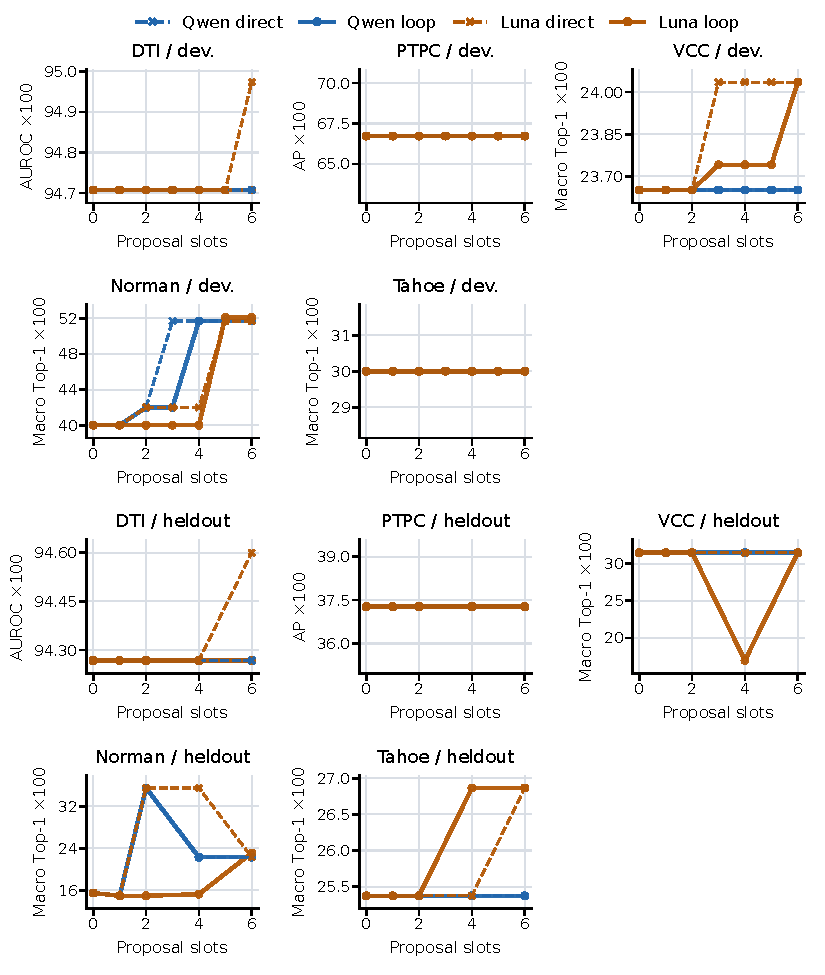
\includegraphics[width=\linewidth]{assets/completed_short6_search.pdf}
\caption{Development selection (upper panels) and held-out performance (lower panels) in the 12-design, six-slot protocol across all five endpoints. Each valid proposal receives the same full fitting schedule; failed slots still consume research budget. Slot 0 is initialization. Held-out curves evaluate the development-selected checkpoints at every prespecified prefix.}
\label{fig:completed-short-dev}
\end{figure}

\clearpage
\subsection*{B.4 Extended search and task-dependent saturation}
The extended study increases the design library to 36 configurations: three learning rates, three weight decays, two server-momentum values and two residual-head settings. It runs 24 proposal slots for both backends and modes on PTPC, VCC, Norman and Tahoe. Prefixes are 0, 1, 2, 4, 6, 8, 12, 16, 20 and 24. The settings for initialization, full candidate fitting, development selection and invalid-slot accounting are otherwise unchanged. DTI's backend comparison is the completed six-slot study in B.3; it is not part of this extended protocol.

\begin{table}[htbp]
\centering\small
\setlength{\tabcolsep}{4pt}
\begin{tabularx}{\linewidth}{@{}Xlrrrrr@{}}
\toprule
Task & Proposer & Fixed & Direct@6 & Loop@6 & Direct@24 & Loop@24 \\
\midrule
PTPC & Luna & \textbf{37.27} & \textbf{37.27} & \textbf{37.27} & \textbf{37.27} & \textbf{37.27} \\
PTPC & Qwen & \textbf{37.27} & \textbf{37.27} & \textbf{37.27} & \textbf{37.27} & \textbf{37.27} \\
VCC & Luna & \textbf{31.50} & 16.94 & 16.94 & 20.23 & 20.01 \\
VCC & Qwen & \textbf{31.50} & \textbf{31.50} & \textbf{31.50} & 19.61 & 19.61 \\
Norman & Luna & 15.48 & \textbf{35.48} & 23.11 & 23.11 & 23.11 \\
Norman & Qwen & 15.48 & \textbf{22.30} & \textbf{22.30} & \textbf{22.30} & \textbf{22.30} \\
Tahoe & Luna & 25.37 & 13.43 & \textbf{26.87} & 13.43 & 13.43 \\
Tahoe & Qwen & 25.37 & \textbf{26.87} & \textbf{26.87} & 13.43 & 13.43 \\
\bottomrule
\end{tabularx}
\caption{Extended 36-design/24-slot heldout results. Four light endpoints, seed 61; no native DTI 24-slot result is implied. All displayed budgets are prefixes of this single protocol; they are not selected by test performance. Every candidate uses 100 rounds. Scores use each original task metric $\times100$; bold marks the best displayed score within a row, including ties.}
\label{tab:completed-long24}
\end{table}

\begin{table}[htbp]
\centering\small
\setlength{\tabcolsep}{4pt}
\begin{tabularx}{\linewidth}{@{}Xlrrrrr@{}}
\toprule
Task & Proposer & Dev. target & First D/L & Last gain D/L & Last retain D/L & Valid D/L \\
\midrule
PTPC & Luna & 66.72 & 0/0 & 0/0 & 0/0 & 24/24 \\
PTPC & Qwen & 66.72 & 0/0 & 0/0 & 0/0 & 19/14 \\
VCC & Luna & 27.68 & 16/9 & 16/10 & 16/10 & 24/24 \\
VCC & Qwen & 24.83 & 18/23 & 18/23 & 18/23 & 11/16 \\
Norman & Luna & 52.10 & 22/4 & 22/4 & 22/7 & 24/24 \\
Norman & Qwen & 51.70 & 2/5 & 2/5 & 22/19 & 15/12 \\
Tahoe & Luna & 35.00 & 5/13 & 5/13 & 5/13 & 24/24 \\
Tahoe & Qwen & 35.00 & 18/14 & 18/14 & 18/14 & 14/15 \\
\bottomrule
\end{tabularx}
\caption{Extended 36-design/24-slot search dynamics. Four light endpoints, seed 61; no native DTI 24-slot result is implied. D/L means direct/loop. The common target is the lower of the two terminal development primary scores, so it is attainable by both runs; first records its earliest attainment. Last gain is the last strictly improving primary-score slot; last retain also includes loss-tiebreak selections. These are retrospective diagnostics, not stopping rules. Slot 0 is initialization.}
\label{tab:completed-dynamics-long24}
\end{table}


Luna produces valid designs in all 192 attempted slots, and Qwen in 116 of 192. Across 16 mode trajectories, the primary development score is unchanged in the final eight slots in 12 cases; the full score/loss selection key is unchanged in ten. Each trajectory retains 11--24 unvisited designs. A plateau therefore characterizes finite-budget search with a particular backend, rather than exhaustion of the design space.

Table~\ref{tab:completed-dynamics-long24} measures the first slot attaining the smaller terminal development score within each direct/loop pair, a common target reached by both modes. Luna reaches Norman's common target earlier with feedback (4 versus 22 slots), whereas direct search reaches Tahoe's target earlier (5 versus 13). Proteomics retains the initial design. Table~\ref{tab:completed-norman-events} connects Norman's trajectory to concrete configuration changes: reducing the learning rate to $10^{-4}$ gives an early development gain, and removing the residual head reaches the final primary-score target. Subsequent loss-tiebreak selections can change the retained design without increasing that primary score.


The eight terminal held-out pairs give seven ties and one decrease with feedback (VCC/Luna, $-0.22$ points). Within this extended protocol, Qwen's VCC held-out Top-1 decreases from 31.50 at slot 6 to 19.61 at slot 24 while development selection improves. This separates the speed of finding a strong development design from generalization of the selected predictor. The complete development and held-out curves support task-specific budget analysis alongside the proposal-validity and remaining-space diagnostics.

\begin{figure}[htbp]
\centering
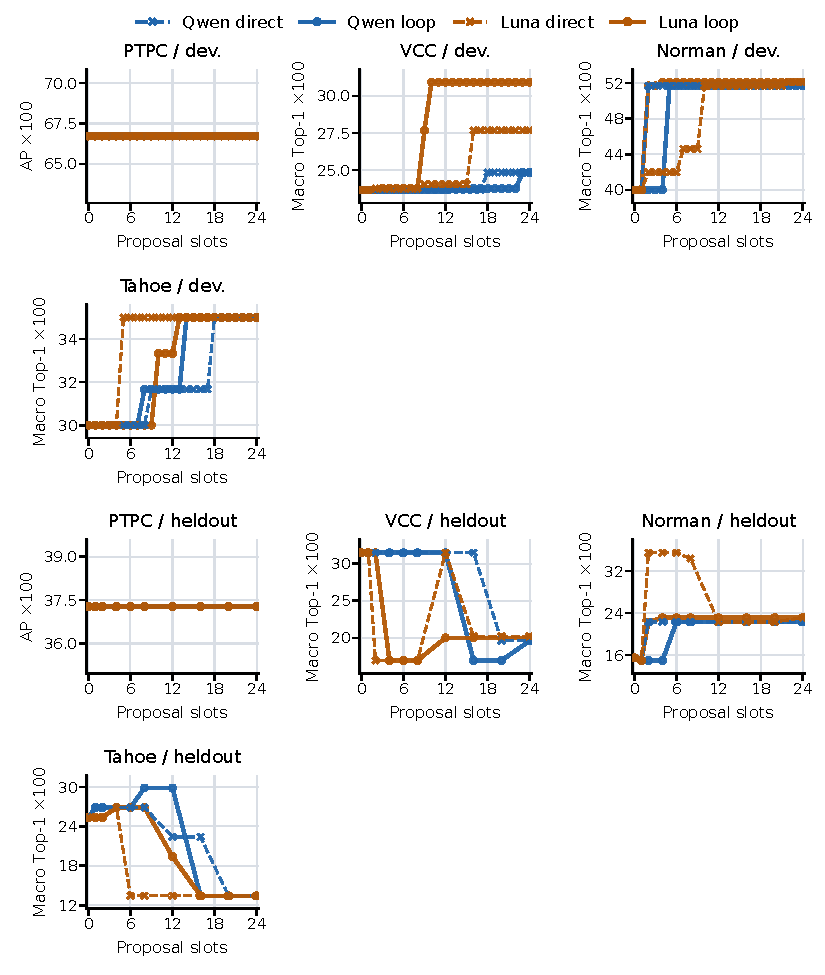
\includegraphics[width=\linewidth]{assets/completed_long24_search.pdf}
\caption{Development selection (upper panels) and held-out performance (lower panels) in the separate 36-design, 24-slot protocol on four endpoints. Curves are paired within the same backend, initialization and design space. Score plateaus may still include loss-tiebreak selections. All prespecified prefixes are displayed. Six-slot points here belong to this 36-design protocol, not the separate 12-design experiment.}
\label{fig:completed-long-dev}
\end{figure}

\clearpage
\subsection*{B.5 Executed designs and proposal traces}
Tables~\ref{tab:completed-menu-short6} and \ref{tab:completed-menu-long24} decode the two design libraries. Tables~\ref{tab:completed-trace-short6} and \ref{tab:completed-trace-long24} retain all 504 attempted proposal slots and their acceptance decisions: 120 slots in the short protocol and 384 in the extended protocol. The accompanying machine-readable trace additionally records each proposal's full configuration, changes from the incumbent and measured development score. Together with the prefix curves, these records connect research decisions to both the executable intervention and its observed outcome.

\begin{table}[htbp]
\caption{All retained proposals for the Norman/Luna extended 36-design, 24-slot study, seed 61. The two modes share initialization and first proposal. lr, wd, m and R denote learning rate, weight decay, server momentum and residual-head indicator. Development selection is followed by evaluation at every prespecified heldout prefix; the full attempted-slot trace is retained separately.}
\label{tab:completed-norman-events}
\centering\small
\setlength{\tabcolsep}{4pt}
\begin{tabularx}{\linewidth}{@{}llXr@{}}
\toprule
Mode & Slot & Executed configuration & Dev. Top-1 \\
\midrule
Direct & 0 & Common initial recipe & 40.00 \\
Direct & 1 & lr=0.001, wd=0.001, m=0, R=1 & 40.00 \\
Direct & 2 & lr=0.001, wd=0.001, m=0.9, R=1 & 42.00 \\
Direct & 7 & lr=0.001, wd=0.01, m=0.9, R=1 & 44.60 \\
Direct & 10 & lr=0.0001, wd=0, m=0, R=1 & 51.70 \\
Direct & 11 & lr=0.0001, wd=0.001, m=0, R=1 & 51.70 \\
Direct & 22 & lr=0.0001, wd=0.001, m=0, R=0 & 52.10 \\
Loop & 0 & Common initial recipe & 40.00 \\
Loop & 1 & lr=0.001, wd=0.001, m=0, R=1 & 40.00 \\
Loop & 2 & lr=0.0001, wd=0.001, m=0, R=1 & 51.70 \\
Loop & 4 & lr=0.0001, wd=0.001, m=0, R=0 & 52.10 \\
Loop & 7 & lr=0.0001, wd=0, m=0, R=0 & 52.10 \\
\bottomrule
\end{tabularx}
\end{table}

\begin{table}[htbp]
\caption{Twelve executable configurations for the short6 protocol. Every design has proximal coefficient zero. A trace design ID uniquely identifies these parameter changes; the task-specific prediction interface remains fixed.}
\label{tab:completed-menu-short6}
\centering\small
\setlength{\tabcolsep}{4pt}
\begin{tabularx}{\linewidth}{@{}Xrrrr@{}}
\toprule
Design & Learning rate & Weight decay & Server momentum & Residual head \\
\midrule
D00 & 0.001 & 0.001 & 0 & No \\
D01 & 0.0001 & 0.001 & 0 & No \\
D02 & 0.01 & 0.001 & 0 & No \\
D03 & 0.001 & 0 & 0 & No \\
D04 & 0.001 & 0.01 & 0 & No \\
D05 & 0.001 & 0.001 & 0.9 & No \\
D06 & 0.001 & 0.001 & 0 & Yes \\
D07 & 0.001 & 0.001 & 0.9 & Yes \\
D08 & 0.0001 & 0.001 & 0 & Yes \\
D09 & 0.0001 & 0.001 & 0.9 & Yes \\
D10 & 0.01 & 0.01 & 0 & No \\
D11 & 0.001 & 0.01 & 0 & Yes \\
\bottomrule
\end{tabularx}
\end{table}

\begin{table}[htbp]
\centering\small
\setlength{\tabcolsep}{4pt}
\begin{tabularx}{\linewidth}{@{}Xrrrr@{}}
\toprule
Design & Learning rate & Weight decay & Server momentum & Residual head \\
\midrule
L0W0M0R0 & 0.0001 & 0 & 0 & No \\
L0W0M0R1 & 0.0001 & 0 & 0 & Yes \\
L0W0M1R0 & 0.0001 & 0 & 0.9 & No \\
L0W0M1R1 & 0.0001 & 0 & 0.9 & Yes \\
L0W1M0R0 & 0.0001 & 0.001 & 0 & No \\
L0W1M0R1 & 0.0001 & 0.001 & 0 & Yes \\
L0W1M1R0 & 0.0001 & 0.001 & 0.9 & No \\
L0W1M1R1 & 0.0001 & 0.001 & 0.9 & Yes \\
L0W2M0R0 & 0.0001 & 0.01 & 0 & No \\
L0W2M0R1 & 0.0001 & 0.01 & 0 & Yes \\
L0W2M1R0 & 0.0001 & 0.01 & 0.9 & No \\
L0W2M1R1 & 0.0001 & 0.01 & 0.9 & Yes \\
L1W0M0R0 & 0.001 & 0 & 0 & No \\
L1W0M0R1 & 0.001 & 0 & 0 & Yes \\
L1W0M1R0 & 0.001 & 0 & 0.9 & No \\
L1W0M1R1 & 0.001 & 0 & 0.9 & Yes \\
L1W1M0R0 & 0.001 & 0.001 & 0 & No \\
L1W1M0R1 & 0.001 & 0.001 & 0 & Yes \\
L1W1M1R0 & 0.001 & 0.001 & 0.9 & No \\
L1W1M1R1 & 0.001 & 0.001 & 0.9 & Yes \\
L1W2M0R0 & 0.001 & 0.01 & 0 & No \\
L1W2M0R1 & 0.001 & 0.01 & 0 & Yes \\
L1W2M1R0 & 0.001 & 0.01 & 0.9 & No \\
L1W2M1R1 & 0.001 & 0.01 & 0.9 & Yes \\
L2W0M0R0 & 0.01 & 0 & 0 & No \\
L2W0M0R1 & 0.01 & 0 & 0 & Yes \\
L2W0M1R0 & 0.01 & 0 & 0.9 & No \\
L2W0M1R1 & 0.01 & 0 & 0.9 & Yes \\
L2W1M0R0 & 0.01 & 0.001 & 0 & No \\
L2W1M0R1 & 0.01 & 0.001 & 0 & Yes \\
L2W1M1R0 & 0.01 & 0.001 & 0.9 & No \\
L2W1M1R1 & 0.01 & 0.001 & 0.9 & Yes \\
L2W2M0R0 & 0.01 & 0.01 & 0 & No \\
L2W2M0R1 & 0.01 & 0.01 & 0 & Yes \\
L2W2M1R0 & 0.01 & 0.01 & 0.9 & No \\
L2W2M1R1 & 0.01 & 0.01 & 0.9 & Yes \\
\bottomrule
\end{tabularx}
\caption{Thirty-six executable configurations for the long24 protocol. Every design has proximal coefficient zero. A trace design ID uniquely identifies these parameter changes; the task-specific prediction interface remains fixed.}
\label{tab:completed-menu-long24}
\end{table}

\clearpage
\begingroup\small
\setlength{\tabcolsep}{3pt}
\begin{longtable}{@{}p{0.10\linewidth}p{0.08\linewidth}p{0.08\linewidth}>{\raggedright\arraybackslash}p{0.66\linewidth}@{}}
\caption{Complete proposal trace for short6. Each token is slot:design:decision, with A=retained, R=not retained, I=invalid. Design configurations are decoded in Table~\ref{tab:completed-menu-short6}. All proposed slots, including failures, are retained. Full configuration deltas and development scores are in the accompanying snapshot and TSV.}\label{tab:completed-trace-short6}\\
\toprule Task & Proposer & Mode & Slot:design:decision \\ \midrule\endfirsthead
\toprule Task & Proposer & Mode & Slot:design:decision \\ \midrule\endhead
\bottomrule\endfoot
DTI & Luna & Direct & 1:D06:R; 2:D05:R; 3:D04:R; 4:D07:R; 5:D03:R; 6:D11:A \\[3pt]
DTI & Luna & Loop & 1:D06:R; 2:D08:R; 3:D05:R; 4:D04:R; 5:D03:R; 6:D01:R \\[3pt]
DTI & Qwen & Direct & 1:D06:R; 2:D07:R; 3:D08:R; 4:D09:R; 5:D04:R; 6:D05:R \\[3pt]
DTI & Qwen & Loop & 1:D06:R; 2:D07:R; 3:D08:R; 4:D09:R; 5:D04:R; 6:D05:R \\[3pt]
PTPC & Luna & Direct & 1:D06:R; 2:D05:R; 3:D03:R; 4:D07:R; 5:D04:R; 6:D11:R \\[3pt]
PTPC & Luna & Loop & 1:D06:R; 2:D08:R; 3:D05:R; 4:D04:R; 5:D11:R; 6:D03:R \\[3pt]
PTPC & Qwen & Direct & 1:D06:R; 2:D07:R; 3:D08:R; 4:D09:R; 5:D04:R; 6:D05:R \\[3pt]
PTPC & Qwen & Loop & 1:D06:R; 2:D10:R; 3:D07:R; 4:D08:R; 5:--:I; 6:D09:R \\[3pt]
VCC & Luna & Direct & 1:D06:R; 2:D07:R; 3:D03:A; 4:D04:R; 5:D05:R; 6:D11:R \\[3pt]
VCC & Luna & Loop & 1:D06:R; 2:D04:R; 3:D05:A; 4:D09:R; 5:D02:R; 6:D03:A \\[3pt]
VCC & Qwen & Direct & 1:D06:R; 2:D07:R; 3:D08:R; 4:D09:R; 5:D04:R; 6:D11:R \\[3pt]
VCC & Qwen & Loop & 1:D06:R; 2:D07:R; 3:D10:R; 4:D08:R; 5:D04:R; 6:D09:R \\[3pt]
Norman & Luna & Direct & 1:D06:A; 2:D07:A; 3:D05:R; 4:D03:R; 5:D08:A; 6:D11:R \\[3pt]
Norman & Luna & Loop & 1:D06:A; 2:D11:R; 3:D05:R; 4:D04:A; 5:D01:A; 6:D09:R \\[3pt]
Norman & Qwen & Direct & 1:D06:A; 2:D07:A; 3:D08:A; 4:D09:R; 5:D04:R; 6:D11:R \\[3pt]
Norman & Qwen & Loop & 1:D06:A; 2:D07:A; 3:D11:R; 4:D08:A; 5:D10:R; 6:D05:R \\[3pt]
Tahoe & Luna & Direct & 1:D06:R; 2:D03:R; 3:D05:R; 4:D07:R; 5:D08:R; 6:D11:A \\[3pt]
Tahoe & Luna & Loop & 1:D06:R; 2:D05:R; 3:D04:A; 4:D11:R; 5:D10:R; 6:D03:R \\[3pt]
Tahoe & Qwen & Direct & 1:--:I; 2:D06:R; 3:D07:R; 4:--:I; 5:D08:R; 6:D09:R \\[3pt]
Tahoe & Qwen & Loop & 1:--:I; 2:D06:R; 3:--:I; 4:D07:R; 5:D09:R; 6:D05:R \\[3pt]
\end{longtable}
\endgroup

\begingroup\small
\setlength{\tabcolsep}{3pt}
\begin{longtable}{@{}p{0.10\linewidth}p{0.08\linewidth}p{0.08\linewidth}>{\raggedright\arraybackslash}p{0.66\linewidth}@{}}
\caption{Complete proposal trace for long24. Each token is slot:design:decision, with A=retained, R=not retained, I=invalid. Design configurations are decoded in Table~\ref{tab:completed-menu-long24}. All proposed slots, including failures, are retained. Full configuration deltas and development scores are in the accompanying snapshot and TSV.}\label{tab:completed-trace-long24}\\
\toprule Task & Proposer & Mode & Slot:design:decision \\ \midrule\endfirsthead
\toprule Task & Proposer & Mode & Slot:design:decision \\ \midrule\endhead
\bottomrule\endfoot
PTPC & Luna & Direct & 1:L1W1M1R1:R; 2:L1W1M0R1:R; 3:L1W1M1R0:R; 4:L1W2M1R1:R; 5:L0W1M0R1:R; 6:L1W2M0R0:R; 7:L2W1M0R0:R; 8:L1W0M0R1:R; 9:L1W0M1R0:R; 10:L1W2M0R1:R; 11:L1W0M0R0:R; 12:L1W2M1R0:R; 13:L0W1M1R1:R; 14:L0W1M0R0:R; 15:L1W0M1R1:R; 16:L0W1M1R0:R; 17:L2W1M0R1:R; 18:L0W2M0R0:R; 19:L0W2M0R1:R; 20:L2W1M1R0:R; 21:L2W2M0R1:R; 22:L0W2M1R1:R; 23:L0W0M1R0:R; 24:L0W0M0R1:R \\[3pt]
PTPC & Luna & Loop & 1:L1W1M1R1:R; 2:L1W2M0R0:R; 3:L1W1M0R1:R; 4:L0W1M0R0:R; 5:L1W1M1R0:R; 6:L1W2M0R1:R; 7:L0W0M0R1:R; 8:L1W0M0R1:R; 9:L0W1M0R1:R; 10:L2W1M0R0:R; 11:L2W2M0R1:R; 12:L2W2M0R0:R; 13:L0W1M1R0:R; 14:L0W0M1R0:R; 15:L1W2M1R0:R; 16:L0W1M1R1:R; 17:L1W2M1R1:R; 18:L0W2M1R0:R; 19:L2W1M0R1:R; 20:L0W2M0R0:R; 21:L0W0M0R0:R; 22:L0W2M0R1:R; 23:L2W0M1R1:R; 24:L0W0M1R1:R \\[3pt]
PTPC & Qwen & Direct & 1:L1W0M0R1:R; 2:L0W0M0R1:R; 3:L1W0M1R1:R; 4:L1W1M1R1:R; 5:L1W2M1R1:R; 6:L0W0M1R1:R; 7:L1W1M0R1:R; 8:L0W1M0R1:R; 9:L0W1M1R1:R; 10:L2W2M1R1:R; 11:L2W0M1R1:R; 12:--:I; 13:L1W2M1R0:R; 14:L2W2M0R1:R; 15:--:I; 16:L2W1M1R1:R; 17:--:I; 18:L2W1M0R1:R; 19:--:I; 20:L1W1M1R0:R; 21:--:I; 22:L2W0M0R1:R; 23:L2W2M1R0:R; 24:L0W2M0R1:R \\[3pt]
PTPC & Qwen & Loop & 1:L1W0M0R1:R; 2:L1W0M0R0:R; 3:--:I; 4:L0W0M0R1:R; 5:L0W0M1R1:R; 6:L0W1M1R1:R; 7:--:I; 8:L0W1M0R1:R; 9:L1W1M1R1:R; 10:--:I; 11:--:I; 12:L1W0M1R1:R; 13:L1W1M0R1:R; 14:L2W2M1R1:R; 15:L1W2M1R1:R; 16:--:I; 17:--:I; 18:--:I; 19:L0W2M0R1:R; 20:L1W1M1R0:R; 21:--:I; 22:L1W2M0R1:R; 23:--:I; 24:--:I \\[3pt]
VCC & Luna & Direct & 1:L1W1M0R1:R; 2:L1W1M1R0:A; 3:L1W1M1R1:R; 4:L1W2M0R1:R; 5:L1W2M1R1:R; 6:L1W0M0R1:R; 7:L1W2M1R0:R; 8:L1W2M0R0:R; 9:L1W0M0R0:A; 10:L0W1M0R1:R; 11:L2W1M0R0:R; 12:L1W0M1R0:R; 13:L1W0M1R1:R; 14:L2W1M1R1:R; 15:L2W1M0R1:R; 16:L2W1M1R0:A; 17:L0W1M0R0:R; 18:L0W1M1R1:R; 19:L0W1M1R0:R; 20:L2W2M0R1:R; 21:L0W2M0R1:R; 22:L0W0M0R1:R; 23:L2W0M0R0:R; 24:L0W2M1R1:R \\[3pt]
VCC & Luna & Loop & 1:L1W1M0R1:R; 2:L2W2M0R0:R; 3:L1W1M1R0:A; 4:L0W1M1R0:R; 5:L1W1M1R1:R; 6:L1W0M1R0:R; 7:L1W2M1R0:R; 8:L0W0M1R1:R; 9:L2W1M1R0:A; 10:L2W2M1R0:A; 11:L2W2M1R1:R; 12:L1W2M1R1:R; 13:L1W2M0R0:R; 14:L1W0M0R0:R; 15:L1W0M1R1:R; 16:L2W2M0R1:R; 17:L1W2M0R1:R; 18:L0W1M0R0:R; 19:L1W0M0R1:R; 20:L2W1M0R0:R; 21:L2W1M0R1:R; 22:L0W1M0R1:R; 23:L2W1M1R1:R; 24:L0W0M0R0:R \\[3pt]
VCC & Qwen & Direct & 1:L1W1M1R1:R; 2:L1W1M0R1:R; 3:L0W0M0R1:R; 4:L0W0M1R1:R; 5:--:I; 6:--:I; 7:L0W1M0R1:R; 8:L1W2M1R1:R; 9:--:I; 10:--:I; 11:--:I; 12:L0W1M1R0:R; 13:--:I; 14:--:I; 15:--:I; 16:--:I; 17:--:I; 18:L2W2M1R1:A; 19:L1W0M1R1:R; 20:--:I; 21:--:I; 22:--:I; 23:L0W1M1R1:R; 24:L1W2M0R1:R \\[3pt]
VCC & Qwen & Loop & 1:L1W1M1R1:R; 2:L0W0M1R1:R; 3:L1W0M0R1:R; 4:--:I; 5:L0W0M0R1:R; 6:--:I; 7:L0W1M1R1:R; 8:L0W1M0R1:R; 9:L1W1M0R1:R; 10:L1W2M1R1:R; 11:L1W2M1R0:R; 12:L0W2M0R1:R; 13:L1W1M1R0:A; 14:--:I; 15:L1W0M1R1:R; 16:--:I; 17:--:I; 18:L2W0M1R1:R; 19:--:I; 20:L1W2M0R1:R; 21:--:I; 22:L2W1M1R1:R; 23:L2W2M1R1:A; 24:--:I \\[3pt]
Norman & Luna & Direct & 1:L1W1M0R1:A; 2:L1W1M1R1:A; 3:L1W0M0R1:R; 4:L1W1M1R0:R; 5:L1W0M1R0:R; 6:L1W2M0R1:R; 7:L1W2M1R1:A; 8:L1W2M0R0:R; 9:L1W0M1R1:R; 10:L0W0M0R1:A; 11:L0W1M0R1:A; 12:L1W2M1R0:R; 13:L0W1M1R1:R; 14:L2W1M0R1:R; 15:L1W0M0R0:R; 16:L2W1M0R0:R; 17:L2W1M1R1:R; 18:L2W2M1R1:R; 19:L2W0M0R1:R; 20:L2W2M0R1:R; 21:L2W0M1R1:R; 22:L0W1M0R0:A; 23:L2W1M1R0:R; 24:L0W1M1R0:R \\[3pt]
Norman & Luna & Loop & 1:L1W1M0R1:A; 2:L0W1M0R1:A; 3:L0W1M1R1:R; 4:L0W1M0R0:A; 5:L0W1M1R0:R; 6:L0W2M0R0:R; 7:L0W0M0R0:A; 8:L0W2M0R1:R; 9:L1W0M0R0:R; 10:L0W0M0R1:R; 11:L1W0M0R1:R; 12:L0W0M1R0:R; 13:L1W1M1R0:R; 14:L1W2M0R0:R; 15:L0W2M1R0:R; 16:L0W2M1R1:R; 17:L0W0M1R1:R; 18:L2W1M0R0:R; 19:L1W1M1R1:R; 20:L1W2M0R1:R; 21:L1W2M1R0:R; 22:L2W2M0R0:R; 23:L1W0M1R0:R; 24:L1W0M1R1:R \\[3pt]
Norman & Qwen & Direct & 1:L1W1M0R1:A; 2:L0W0M0R1:A; 3:L0W1M1R1:R; 4:--:I; 5:L1W1M1R1:R; 6:L0W0M1R1:R; 7:--:I; 8:L2W2M1R1:R; 9:L0W1M0R1:A; 10:--:I; 11:L1W2M0R1:R; 12:L1W2M1R1:R; 13:--:I; 14:--:I; 15:--:I; 16:--:I; 17:L2W2M0R1:R; 18:L2W1M0R1:R; 19:L2W0M1R1:R; 20:L2W1M1R1:R; 21:--:I; 22:L0W2M0R1:A; 23:--:I; 24:L1W0M0R1:R \\[3pt]
Norman & Qwen & Loop & 1:L1W1M0R1:A; 2:--:I; 3:--:I; 4:L1W0M0R1:A; 5:L0W0M0R1:A; 6:L1W2M1R1:R; 7:--:I; 8:L0W0M1R1:R; 9:--:I; 10:--:I; 11:--:I; 12:L1W1M1R1:R; 13:--:I; 14:L0W1M1R1:R; 15:L1W2M0R0:R; 16:L1W1M1R0:R; 17:--:I; 18:--:I; 19:L0W1M0R1:A; 20:--:I; 21:L1W2M0R1:R; 22:--:I; 23:--:I; 24:L0W2M1R1:R \\[3pt]
Tahoe & Luna & Direct & 1:L1W1M0R1:R; 2:L1W1M1R1:R; 3:L1W1M1R0:R; 4:L1W2M0R1:A; 5:L1W2M1R1:A; 6:L1W0M0R1:R; 7:L1W0M0R0:R; 8:L1W2M1R0:R; 9:L1W2M0R0:R; 10:L1W0M1R1:R; 11:L0W1M0R0:R; 12:L0W0M0R1:R; 13:L1W0M1R0:R; 14:L0W1M0R1:R; 15:L0W1M1R1:R; 16:L2W1M0R0:R; 17:L0W0M1R1:R; 18:L2W1M1R0:R; 19:L0W1M1R0:R; 20:L2W1M0R1:R; 21:L2W1M1R1:R; 22:L0W2M0R1:R; 23:L2W2M1R1:R; 24:L0W2M1R1:R \\[3pt]
Tahoe & Luna & Loop & 1:L1W1M0R1:R; 2:L1W1M1R0:R; 3:L1W2M0R0:A; 4:L0W2M0R0:R; 5:L1W2M0R1:R; 6:L2W1M0R0:R; 7:L0W1M0R0:R; 8:L0W2M0R1:R; 9:L2W2M0R0:R; 10:L0W2M1R0:A; 11:L0W2M1R1:R; 12:L1W2M1R0:R; 13:L1W2M1R1:A; 14:L0W1M1R1:R; 15:L0W0M1R0:R; 16:L0W1M1R0:R; 17:L0W0M0R0:R; 18:L1W0M1R1:R; 19:L2W1M0R1:R; 20:L0W1M0R1:R; 21:L1W0M0R1:R; 22:L0W0M1R1:R; 23:L0W0M0R1:R; 24:L1W0M0R0:R \\[3pt]
Tahoe & Qwen & Direct & 1:L1W0M0R1:A; 2:L1W1M0R1:R; 3:--:I; 4:--:I; 5:L0W0M0R1:R; 6:--:I; 7:--:I; 8:L1W1M1R1:R; 9:L0W0M1R0:A; 10:L0W0M1R1:R; 11:--:I; 12:L0W1M0R1:R; 13:L1W2M1R0:R; 14:--:I; 15:L2W1M1R1:R; 16:L0W1M1R1:R; 17:L2W2M1R1:R; 18:L1W2M1R1:A; 19:--:I; 20:--:I; 21:L1W2M0R1:R; 22:L1W0M1R1:R; 23:--:I; 24:--:I \\[3pt]
Tahoe & Qwen & Loop & 1:L1W0M0R1:A; 2:--:I; 3:--:I; 4:--:I; 5:L1W1M1R1:R; 6:--:I; 7:L1W1M0R1:R; 8:L1W0M1R1:A; 9:L0W0M1R1:R; 10:L0W0M0R1:R; 11:--:I; 12:--:I; 13:--:I; 14:L1W2M1R1:A; 15:L2W2M1R0:R; 16:L0W1M1R1:R; 17:--:I; 18:L0W1M0R1:R; 19:L0W1M1R0:R; 20:--:I; 21:L1W2M0R1:R; 22:L2W1M1R1:R; 23:L2W2M1R1:R; 24:L0W2M0R1:R \\[3pt]
\end{longtable}
\endgroup



\clearpage
\section*{Appendix C. Public research-controller comparison}
\label{app:public-harness-comparison}
\setcounter{table}{0}
\renewcommand{\thetable}{C.\arabic{table}}
\renewcommand{\theHtable}{C.\arabic{table}}

\subsection*{C.1 Shared biological task interface}
We connect the released research controllers of AI-Scientist-v2 \citep{Yamada2025AIScientistV2} and AI-Researcher \citep{Tang2025AIResearcher} to the same biological fitting and evaluation service used by BioCoLoop. The source versions are \texttt{96bd51617cfd} and \texttt{f9a6f8480860}, respectively \citep{AIScientistV2Code,AIResearcherCode}. Because neither public framework implements our collaborative training and distributed-evaluation protocol, each public controller accesses laboratory 0 only; BioCoLoop accesses all ten laboratories. The controllers otherwise share the original twelve-design library, at most six candidate proposals, 100 training rounds per valid candidate and the same held-out scorer. The service first fits D00 afresh. The submitted design ID is the executable field; its accompanying hypothesis, experiment and expected-effect text records the controller's rationale. Repeated or invalid design requests consume a proposal slot, and a controller may stop its native refinement process before exhausting the cap. Development score and loss select the retained checkpoint under the original selection rule.

AI-Scientist-v2 retains its experiment manager, tree-search paths, experiment reviews and journal. AI-Researcher retains its native idea selection, planning, implementation, review handoffs and iterative experiment analysis. Task-specific prompts direct these controllers to the registered design interface. Executing arbitrary generated code, external retrieval, figure review and manuscript generation are outside this fixed-task experiment. The public controllers use local Qwen2.5-7B-Instruct with temperature 0.7, top-$p$ 0.9 and at most 512 generated tokens per call. Their adapter allows at most 160 model calls and 28,000 input tokens per call. Full model-call counts and token usage accompany each run; equal proposal and candidate-training budgets do not imply equal language-model costs.

\subsection*{C.2 Prediction quality and execution outcomes}
A scored run completes its controller-selected research process under the registered cap, seals development selection and passes independent rescoring of saved held-out predictions. Table~\ref{tab:public-harness-comparison-three-seed} reports the seed-42 comparison. With laboratory-0 access, AI-Scientist-v2 reaches 20.19\% PTPC AP and 21.73\%, 14.15\% and 13.43\% Top-1 on VCC, Norman and Tahoe. AI-Researcher reaches 86.01\% DTI AUROC, 20.17\% PTPC AP and 21.73\%, 25.56\% and 19.40\% Top-1 on the three cell endpoints. BioCoLoop is highest on DTI, proteomics, VCC and Tahoe with 94.60\%, 37.12\%, 31.63\% and 23.88\%, while AI-Researcher is highest on Norman.

AI-Scientist-v2's DTI controller trains D01, D05 and D08 for 100 rounds each; D01 becomes the development incumbent. When the native tree-search advances to its next research stage, its upstream substage generator fails schema validation on all three attempts and the manager raises a pipeline exception before the six-slot selection can be sealed. We report $F_{\mathrm{pipe}}$ rather than evaluating the unsealed incumbent. AI-Researcher completes DTI with six recorded requests, including invalid out-of-menu proposals that consume slots under the prespecified protocol, and retains D00 by development selection.

The held-out scorer runs only after development selection is sealed. For every scored cell, an independent verifier reloads the saved predictions, recomputes the task metric and checks the selected checkpoint and artifact hashes. The DTI rescore differs from the stored metrics by at most $10^{-15}$. Raw model calls, native stage history, candidate requests, selections and verification receipts accompany the runs.

\subsection*{C.3 Task-transport repair}
The final AI-Researcher adaptation removes repeated task packets from stage prompts while retaining the complete current task and measured evidence in each system prompt. Native stage reasoning and tool results are preserved. The text bridge accepts an unambiguous \texttt{parameters} alias for \texttt{arguments} and standard single-tool-call envelopes, without inferring actions or parameter values. Six proposals are a maximum, so the controller may end refinement early. Model weights, context allowance, candidate training and scoring are unchanged. This transport revision is fixed across the five reported endpoints. AI-Scientist-v2's DTI pipeline error is retained as an execution outcome rather than motivating a post-hoc controller repair.


\end{document}
